\documentclass[a4paper,12pt]{book}
\usepackage[utf8]{inputenc}
\usepackage[francais]{babel}
\usepackage[T1]{fontenc}
\usepackage{graphicx}
\usepackage{subcaption}
\usepackage[colorlinks,urlcolor=blue]{hyperref} %hyperlinks
\usepackage{xcolor} %color text
\usepackage[amsthm]{ntheorem} %theorems and co.
\usepackage{amsmath} %mathematical symbols
\usepackage{amssymb} %squares in itemize
\usepackage[page,toc,titletoc,title]{appendix} %appendices
\usepackage{natbib} %bibliography
\usepackage[nottoc,notlot,notlof]{tocbibind} %bind the table of contents to the bibligoraphy
\usepackage{packages/tikz-uml} %UML elements
\usepackage{silence} %silencing warnings
\WarningFilter{latex}{Text page}

%Defining custom commands for relational model
\newcommand{\attr}[1]{\emph{#1}}
\newcommand{\texit}[1]{\#\textsl{#1}}

%Redefining the appendices name to "Annexes" in toc and removing "Annexe" from appendice title
\renewcommand{\appendixtocname}{Annexes}
\appendixtitletocoff

%Defining a new command for the horizontal lines
\newcommand{\HRule}{\rule{\linewidth}{0.5mm}}

%Defining custom environments
\theoremstyle{break}
\newtheorem*{userStory}{User Story}

\theoremstyle{break}
\newtheorem*{definition}{Définition}

\theoremstyle{break}
\newtheorem*{property}{Propriété}

\theoremstyle{break}
\newtheorem*{constraint}{Règle}

\theoremstyle{definition}
\newtheorem*{example}{Exemple}

\theoremstyle{remark}
\newtheorem*{remark}{\textbf{Remarque}}

\begin{document}
\pagestyle{plain}
%----------------------------------------------------------------------------------------
%   TITLE PAGE
%----------------------------------------------------------------------------------------
\begin{titlepage}
\centering
%----------------------------------------------------------------------------------------
%   LOGOS SECTION
%----------------------------------------------------------------------------------------

\includegraphics[scale=0.5]{images/umLogo.png} %Université de Montpellier Logo
\hspace{\fill}

\includegraphics[scale=0.25]{images/fdsLogo.jpg} %Faculté de Sciences Logo
\hspace{\fill}

\includegraphics[scale=0.25]{images/lirmmLogo.png}~\\[2cm] %LIRMM Logo
%----------------------------------------------------------------------------------------
%   HEADING SECTIONS
%----------------------------------------------------------------------------------------
\textsc{\LARGE L3 CMI Informatique}\\[0.5cm]
\textsc{\Large \textbf{HLSE602} -- Projet Annuel CMI}\\[0.25cm]
\textsc{\Large \texttt{LaRuche}}\\[2cm]
%----------------------------------------------------------------------------------------
%   TITLE SECTION
%----------------------------------------------------------------------------------------
\HRule \\[0.4cm]
{\huge \bfseries RAPPORT \#$1$}\\[0.1cm]
\HRule \\[2cm]
%----------------------------------------------------------------------------------------
%   STUDENTS SECTION
%----------------------------------------------------------------------------------------
\begin{minipage}{0.5\textwidth}
\centering \large
\textbf{Bachar \textsc{Rima}}\\
\textbf{Othmane \textsc{Farajallah}}\\
\textbf{Wissem \textsc{Soussi}}
\end{minipage} \\[2cm]
%----------------------------------------------------------------------------------------
%   SUPERVISORS SECTION
%----------------------------------------------------------------------------------------
\begin{minipage}[b]{0.5\textwidth}
\begin{flushleft} \large
\emph{Responsable CMI Informatique :} \\
Anne-Elisabeth \textsc{Baert} \\
\end{flushleft}
\end{minipage}
~
\begin{minipage}[b]{0.4\textwidth}
\begin{flushright} \large
\emph{Encadrant :}\\
Eric \textsc{Bourreau}
\end{flushright}
\end{minipage}\\[1.5cm]
%----------------------------------------------------------------------------------------
%   DATE SECTION
%----------------------------------------------------------------------------------------
{\large \today}\\[1cm]
\hspace{\fill}
\vfill % Fill the rest of the page with whitespace
\end{titlepage}
%----------------------------------------------------------------------------------------
%   TABLE OF CONTENTS
%----------------------------------------------------------------------------------------
{
  \hypersetup{linkcolor=black}
  \tableofcontents
}
%----------------------------------------------------------------------------------------
%   INTRODUCTION
%----------------------------------------------------------------------------------------
\chapter{Introduction}
%----------------------------------------------------------------------------------------
%   CONTEXTE DU STAGE
%----------------------------------------------------------------------------------------
\section{Contexte du projet}
Dans ce rapport, nous nous consacrons à la description détaillée de la phase de conception du projet intitulé \texttt{LaRuche} à effectuer au sein du \textbf{LIRMM} (\textbf{L}aboratoire d'\textbf{I}nformatique, de \textbf{R}obotique et de \textbf{M}icroélectronique de \textbf{M}ontpellier) dans le cadre du module \textbf{HLSE602 -- Projet Annuel CMI} de la $3$\ieme{} année de licence en \textbf{CMI} (\textbf{C}ursus \textbf{M}aster \textbf{I}ngénierie).

Le projet se déroule sous l'encadrement de Mme Anne-Elisabeth Baert, enseignante/chercheuse au sein du LIRMM dans l'équipe \textbf{MAORE} (\textbf{M}éthodes \textbf{A}lgorithmes pour l'\textbf{O}rdonnancement et les \textbf{Ré}seaux) \citep{AEBPres}, en tant que responsable de la formation CMI informatique et M. Eric Bourreau, enseignant/chercheur au sein du LIRMM dans la même équipe \textbf{MAORE} \citep{EricBourreauPres}, en tant que responsable pédagogique et encadrant du projet.

Le sujet du projet couvre la création d'un site web dédié comme interface de communication entre vendeurs de produits locaux et leurs clients. Il est inspiré du site \og \href{https://laruchequiditoui.fr/fr}{La Ruche Qui Dit Oui} \fg traitant le même thème et répondant aux mêmes besoins, mais cherche à faire les choses d'une façon différente, surtout au niveau de la logistique et de l'architecture du site, afin de fournir une vision différente, voire plus optimisée de la gestion des interactions directes entre clients et vendeurs.

Nous commencerons ce rapport en annonçant le contexte du projet, puis nous présenterons LIRMM, les problématiques adressées et traitées dans le cadre du projet, la méthodologie adoptée pour modéliser le problème et y proposer des solutions ainsi que les outils de modélisation et le planning prévisionnel pour répartir les tâches à effectuer dans un cadre spatio-temporel valable. Après, nous présenterons l'aperçu d'un entretien déroulé avec un client potentiel afin d'inclure ses besoins dans le cahier des charges de notre projet et de modifier notre modélisation de manière à y répondre. Enfin, nous conclurons en discutant l'implémentation prévue de l'application modélisée et les perspectives.
%----------------------------------------------------------------------------------------
%   PRÉSENTATION DU LIRMM
%----------------------------------------------------------------------------------------
\section{Présentation du LIRMM}
\og Le [...] – LIRMM – est une unité mixte de recherche, dépendant conjointement de l'Université Montpellier et du Centre National de la Recherche Scientifique [(CNRS)]. Il est situé sur le Campus Saint-Priest de l'UM [(Figure \ref{fig:lirmmPhoto})].

\begin{figure}[!ht]
  \centering
  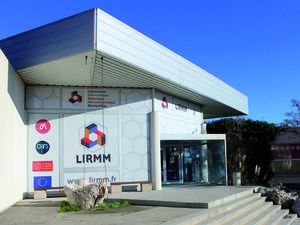
\includegraphics[scale=0.9]{images/lirmmPhoto.jpg}
  \caption{bâtiment 3 du LIRMM, Campus St. Priest}
  \label{fig:lirmmPhoto}
\end{figure}

Les travaux sont menés dans trois départements scientifiques de recherche, [(L’Informatique, La Robotique, et La Microélectronique)] eux-mêmes organisés en \og équipes-projet \fg.

Les recherches menées au LIRMM trouvent généralement une finalisation dans des domaines applicatifs aussi divers que la biologie, la chimie, les télécommunications, la santé, l'environnement... et dans les domaines propres du laboratoire : l'informatique, l'électronique et l'automatique.

Ses activités de recherche [le] positionnent [...] pleinement au coeur des sciences et technologies de l’information, de la communication et des systèmes. [En particulier,] les thématiques du département Informatique s’étendent des frontières des mathématiques à la recherche appliquée : algorithmique des graphes, bioinformatique, cryptographie, réseaux, bases de données et systèmes d'information [...], génie logiciel [...], intelligence artificielle [...], interaction homme-machine [...]. \fg{} \citep{lirmmPres}
%----------------------------------------------------------------------------------------
%   PROBLÈME, MÉTHODOLOGIE, OUTILS ET PLANNING
%----------------------------------------------------------------------------------------
\chapter{Problème, Méthodologie, Outils et Planning}
%----------------------------------------------------------------------------------------
%   PROBLÈME
%----------------------------------------------------------------------------------------
\section{Problème}
Les gens cherchent de \textit{plus en plus} d'acheter des produits frais minimisant les étapes de \textit{processing}, alors que les producteurs cherchent à se libérer des centres d’achat et des intermédiaires de distribution.

Dans l’esprit du site francais \href{https://laruchequiditoui.fr/fr}{LaRucheQuiDitOui}, on souhaite implémenter une interface sous forme d'un \textbf{site web} permettant, au premier, aux producteurs de vendre leurs produits \textbf{directement} aux consommateurs en se regroupant en des endroits précis afin de proposer d'offres diversifiés de leurs produits.

Le site web offrera ainsi \textbf{tout le nécessaire} aux consommateurs pour effectuer des commandes prépayées et précisera en suite les points de collecte de produits les plus proches. D'autre part, le site offrera aussi aux fournisseurs la possibilité d'organiser ces points, de gérer la mise à jour des
stocks et la mise en vente/prise de commandes par les clients, en se basant sur des algorithmes d'optimisation aidant à l'organisation de la logistique, à la préparation/facturation des commandes et à la redistribution des produits entre les différents producteurs voisins.
%----------------------------------------------------------------------------------------
%   MÉTHODOLOGIE
%----------------------------------------------------------------------------------------
\section{Méthodologie}
Dans le but d'assurer la meilleure gestion de nos ressources en offrant le plus de fonctionnalités possibles aux utilisateurs tout en implémentant progressivement leurs requis et faisant sortir des versions fonctionnelles du site après avoir tester les parties implémentées après chaque itération de développement, nous avons opté pour une approche basée sur les \textbf{méthodes agiles} de développement et \textbf{XP}\footnote{\textit{eXtreme Programming}}.

En effet, la méthodologie de développement proposée par les méthodes agiles étant de plus en plus prépondérante en génie logiciel, nous avons décidé d'en profiter pour la modélisation et l'implémentation ultérieure de notre site web pour assurer le plus de flexibilité et d'extensibilité possible lors du dialect développeurs/utilisateurs permettant de répondre efficacement aux besoins des utilisateurs.
%----------------------------------------------------------------------------------------
%   OUTILS
%----------------------------------------------------------------------------------------
\section{Outils}
Pour garantir une bonne modélisation du projet, en cohérence avec l'approche de la méthodologie discutée précédemment, on aura besoin d'expliciter les spécifications fonctionnelles et organisationnelles de notre projet. Ainsi, on aura recours aux outils suivants :
\begin{description}
  \item[\textit{user stories}]{des requis fournis par les utilisateurs décrivant en langage naturel les fonctionnalités qu'il souhaitent avoir dans le site.}
  \item[diagrammes de cas d'usage]{des diagrammes dynamiques, souvent utilisés en \textbf{UML} pour décrire en haut niveau les fonctionnalités d'un système, en se servant de notions telles que \textbf{acteurs}, \textbf{cas d'usage}, \textbf{systèmes} et les \textbf{relations} entre chacune de ces entités.}
  \item[modèle EA]{un modèle \textbf{conceptuel} utilisé pour décrire les entités du projet ainsi que les associations décrivant leurs relations et comportements.}
  \item[schéma de base de données]{schéma en modèle \textbf{relationnel} composé des schémas des relations et des contraintes d'intégrité sur l'ensemble des relations, traduit généralement à partir du \textbf{modèle EA} et servant comme \textbf{modèle logique} lors de l'implémentation de la \textbf{base de données}.}
  \item[\textit{mockup storyboard}]{document de haut niveau offrant un moyen pour schématiser l'utilisation d'un projet, en positionant les différents éléments le composant, sans rentrer dans les détails de leur fonctionnement (cf. Annexe \ref{app:storyoard}).}
\end{description}
%----------------------------------------------------------------------------------------
%   CONCEPTION
%----------------------------------------------------------------------------------------
\chapter{Conception}
%----------------------------------------------------------------------------------------
%   USER STORIES ET DIAGRAMMES DE CAS D'USAGE
%----------------------------------------------------------------------------------------
\section{\textit{User Stories} et Diagrammes de cas d'usage}
Dans cette section nous illustrons les \textit{user stories} que nous avons rédigées pour identifier les fonctionnalités du système conçu, ainsi que les diagrammes de cas d'usage de quelques fonctionnalités parmi celles illustrées.

Les \textit{user stories} de cette section seront implémentées dans la $1$\iere{} version du site, désignant les \textbf{fonctionnalités de base}, assimilant notre site en une \textbf{vitrine de réservation de produits} et non pas une \textbf{vitrine commerciale d'achats}. Cependant, nous avons inclus dans nos analyses des \textit{user stories} désignant des \textbf{fonctionnalités supplémentaires avancées}, mais pour rester en accord avec la philosophie de \textbf{XP}, elles seront traitées dans les versions du site à venir. Toutefois, leurs \textit{user stories} seront incluses dans la section des \textbf{Perspectives} (cf. Section \ref{sec:perspectives}).

\subsection{Page d'accueil du site}
\begin{userStory}[Création de compte]
\textbf{En tant qu'utilisateur {\color{green}client}/{\color{red} fournisseur}}, je souhaite avoir mon \textbf{propre compte},\\
\indent
\textbf{dans le but de} visualiser le site selon mes \textbf{préférences} et avois accès à mon \textbf{historique d'achats}.
\end{userStory}

\begin{userStory}[Client/Fournisseur avec le même compte utilisateur]
\textbf{En tant qu'utilisateur}, je souhaite avoir la possibilité de consulter le site en tant que \textbf{{\color{green}client acheteur}} et/ou \textbf{{\color{red} fournisseur}} (\textit{si besoin}),\\
\indent
\textbf{dans le but de} profiter du site en tant que consommateur et/ou producteur, sans besoin de me déconnecter de mon compte à chaque fois que je souhaite échanger entre les deux modes d'utilisation.
\end{userStory}

\begin{userStory}[Menu de navigation du pied de page]
En tant qu'\textbf{utilisateur} \textbf{{\color{green} client}/{\color{red} fournisseur}}, je souhaite consulter les informations pertinentes au site depuis un \textbf{menu de navigation placé dans le pied de page},\\
\indent
\textbf{dans le but de} m'informer sur l'utilisation du site (\textbf{FAQ}), les \textbf{termes et conditions d'utilisation}, les \textbf{créateurs du site}, $\dots$.
\end{userStory}

\begin{figure}[!ht]
  \centering
  \begin{tikzpicture}
    \umlactor{User}
    \umlactor[x=12, y=-1]{Database}
    \begin{umlsystem}[x=4, fill=red!10]{index page}
      \umlusecase{Sign-up}
      \umlusecase[y=-2]{Sign-in}
      \umlusecase[x=4, width=1.5cm]{Create database entry}
      \umlusecase[x=4, y=-3, width=1.5cm]{Verify credentials}
      \umlusecase[y=-4]{Footer menu}
    \end{umlsystem}
    \umlassoc{User}{usecase-1}
    \umlassoc{User}{usecase-2}
    \umlassoc{User}{usecase-5}
    \umlassoc{Database}{usecase-3}
    \umlassoc{Database}{usecase-4}
    \umlinclude{usecase-1}{usecase-3}
    \umlinclude{usecase-2}{usecase-4}
    \umlinclude{usecase-3}{usecase-4}
  \end{tikzpicture}
  \caption{Diagramme de cas d'usage des fonctionnalités de la page d'accueil du site}
  \label{fig:index_page_case_diagram}
\end{figure}

\subsection{Page d'accueil de l'utilisateur}
\begin{userStory}[Paramètres personnalisés]
\textbf{En tant qu'utilisateur {\color{green}client}/{\color{red}fournisseur}}, je souhaite visualiser des informations sur ma \textbf{page d'accueil} concernant mes intérêts (produits, vendeurs, ruches) selon mes \textbf{préférences spécifiées} dans les \textbf{paramètres} de mon compte et l'\textbf{historique de mes achats/ventes}.\\
\indent
\textbf{dans le but d'}interagir avec des données pertinentes à \textbf{mes intérêts}, sans avoir besoin de toujours les rechercher moi-même, tout en prenant en compte mes \textbf{paramètres de confidentialité}.
\end{userStory}

\begin{userStory}[Résultats de recherche]
\textbf{En tant qu'utilisateur {\color{green}client}/{\color{red}fournisseur}}, je souhaite visualiser des informations sur les produits/vendeurs/ruches dans les résultats de recherche,\\
\indent
\textbf{dans le but d'}avoir \textbf{suffisamment d'information} sur les \textbf{produits} avant de les acheter ou sur les \textbf{fournisseurs}/\textbf{ruches} pour les \textbf{consulter}.
\end{userStory}

\begin{userStory}[Paramètres de recherche]
\textbf{En tant qu'utilisateur {\color{green}client}/{\color{red}fournisseur}}, je souhaite \textbf{trier} mes \textbf{résultats de recherche} selon des \textbf{paramètres}, tels que informations sur les stocks, date de récolte, date d'expiration, prix, proximité, popularité, fournisseur, catégorie, liste de produits similaires, $\dots$\\
\indent
\textbf{dans le but de personnaliser} mes \textbf{résultats de recherche} selon mes besoins.
\end{userStory}

\begin{userStory}[Ergonomie de recherche]
\textbf{En tant qu'utilisateur {\color{green}client}/{\color{red}fournisseur}}, je souhaite avoir lors d'une recherche quelques \textbf{fonctionnalités} telles que la \textbf{complétion automatique}, la \textbf{mise en évidence}, les \textbf{animations}/\textbf{effets visuels}, $\dots$\\
\indent
\textbf{dans le but de} rendre ma recherche \textbf{plus rapide}, plus facile, et \textbf{plus ergonomique}.
\end{userStory}

\begin{figure}[!ht]
  \centering
  \begin{tikzpicture}
    \setcounter{tikzumlUseCaseNum}{0}
    \umlactor{User}
    \umlactor[y=-4]{Vendor}
    \umlactor[x=10, y=-3]{Database}
    \begin{umlsystem}[x=4, fill=green!10]{home page}
      \umlusecase[x=1, width=3cm]{Display Products/Collection Events}
      \umlusecase[x=1, y=-3, width=3cm]{Display Stock/Hive Information}
      \umlusecase[x=1, y=-5]{Search}
      \umlusecase[x=1, y=-7]{Footer menu}
    \end{umlsystem}
    \umlinherit{Vendor}{User}
    \umlextend{usecase-2}{usecase-1}
    \umlassoc{User}{usecase-1}
    \umlassoc{Vendor}{usecase-2}
    \umlassoc{User}{usecase-3}
    \umlassoc{User}{usecase-4}
    \umlassoc{Database}{usecase-1}
    \umlassoc{Database}{usecase-3}
  \end{tikzpicture}
  \caption{Diagramme de cas d'usage des fonctionnalités de la page d'accueil de l'utilisateur}
  \label{fig:home_page_use_case_diagram}
\end{figure}

\begin{figure}[!ht]
  \centering
  \begin{tikzpicture}
    \setcounter{tikzumlUseCaseNum}{0}
    \umlactor[x=-5]{User}
    \umlactor[x=7]{Database}
    \begin{umlsystem}[x=2, fill=green!10]{home page}
      \umlusecase[x=-1]{Search}
      \umlusecase[x=-3.5, y=-3, width=2cm]{Choose Search Parameters}
      \umlusecase[x=1.5, y=-3, width=2cm]{Activate Search Features}
    \end{umlsystem}
    \umlextend[name=ext]{usecase-2}{usecase-1}
    \umlextend[name=ext2]{usecase-3}{usecase-1}
    \umlassoc{User}{usecase-1}
    \umlassoc{User}{usecase-2}
    \umlassoc{User}{usecase-3}
    \umlassoc{Database}{usecase-1}
    \umlassoc{Database}{usecase-2}
    \umlassoc{Database}{usecase-3}
    \umlnote[x=-5.5, y=-2.8, width=2.5cm]{ext-1}{default parameters, else check what parameters to use}
    \umlnote[x=7.5, y=-2.8, width=2.5cm]{ext2-1}{activated by default, else disable in settings}
  \end{tikzpicture}
  \caption{Diagramme de cas d'usage des fonctionnalités de recherche}
  \label{fig:search_use_case_diagram}
\end{figure}

\newpage

\subsection{Communication}
\begin{userStory}[Chat Client $\leftrightarrows$ Fournisseur ou Fournisseur $\leftrightarrows$ Client/Fournisseur]
\textbf{En tant qu'utilisateur}, je souhaite communiquer avec d'autres \textbf{utilisateurs}\footnote{il n'y a pas de chat entre deux utilisateurs {\color{green}clients}} (\textbf{{\color{green}client}} $\leftrightarrows$ \textbf{{\color{red}fournisseur}} ou \textbf{{\color{red}fournisseur}} $\leftrightarrows$ \textbf{{\color{green}client}/{\color{red}fournisseur}} via un \textbf{environnement privé de chat},\\
\indent
\textbf{dans le but de} me renseigner davantage sur certains produits, ruches, $\dots$
\end{userStory}

\begin{figure}[!ht]
  \centering
  \begin{tikzpicture}
    \setcounter{tikzumlUseCaseNum}{0}
    \umlactor{User}
    \umlactor[x=8]{Vendor}
    \begin{umlsystem}[x=4, fill=green!10]{home page}
      \umlusecase{Chat privately}
    \end{umlsystem}
    \umlassoc{User}{usecase-1}
    \umlassoc{Vendor}{usecase-1}
  \end{tikzpicture}
  \caption{Diagramme de cas d'usage de la fonctionnalité de chat}
  \label{fig:instant_messaging_use_case_diagram}
\end{figure}

\subsection{Produits \} Logistiques}
\subsubsection{Gestion de Produits}
\begin{userStory}[Avis sur les produits]
\textbf{En tant qu'utilisateur}, je souhaite \textbf{consulter des avis} (\textbf{{\color{green}client}/{\color{red}fournisseur}}) sur les \textbf{produits} et d'en \textbf{rédiger} (\textbf{{\color{green}client} uniquement}),\\
\indent
\textbf{dans le but d'}avoir plus d'\textbf{informations sur ces produits avant de les acheter} et \textbf{évaluer mon expérience} pour la transmettre aux prochains acheteurs.
\end{userStory}

\begin{userStory}[Définition et stockage de produits]
\textbf{En tant qu'utilisateur {\color{red}fournisseur}}, je souhaite \textbf{définir} ma \textbf{séléction de produits} selon des \textbf{informations caractéristiques} à fournir dans des \textbf{formulaires},\\
\indent
\textbf{dans le but de} maximiser la transparence de mes produits pour gagner la fidelité de mes clients, tout en \textbf{gérant} (création, modification, ajout, suppression) ma sélection à travers le site.
\end{userStory}

\begin{userStory}[Offres de Paniers]
\textbf{En tant qu'utilisateur {\color{red}fournisseur}}, je souhaite créer des \textbf{offres de paniers de produits différents},\\
\indent
\textbf{dans le but de} diversifier ma stratégie de marketing et augmenter mes profits.
\end{userStory}

\begin{userStory}[Rapports de suivi périodiques]
\textbf{En tant qu'utilisateur {\color{red}fournisseur}}, je souhaite consulter \textbf{périodiquement} des \textbf{rapports de suivi} sur la progression de mes \textbf{transactions}, mes \textbf{produits}, et mes \textbf{stocks},\\
\indent
\textbf{dans le but d'}analyser le marché et définir par conséquent ma méthodologie d'offre et de demande.
\end{userStory}

\begin{figure}[!ht]
  \centering
  \begin{tikzpicture}
    \setcounter{tikzumlUseCaseNum}{0}
    \umlactor{User}
    \umlactor[y=-3]{Client}
    \umlactor[x=8]{Database}
    \begin{umlsystem}[x=4, fill=green!10]{home page}
      \umlusecase{Search}
      \umlusecase[y=-2, width=2cm]{Search for Products}
      \umlusecase[y=-4]{Review Products}
    \end{umlsystem}
    \umlinherit{Client}{User}
    \umlextend{usecase-2}{usecase-1}
    \umlextend[name=ext]{usecase-3}{usecase-2}
    \umlassoc{User}{usecase-1}
    \umlassoc{Client}{usecase-3}
    \umlassoc{Database}{usecase-1}
    \umlassoc{Database}{usecase-3}
    \umlnote[x=9, y=-3]{ext-1}{Only if the user is a client having already purchased the product}
  \end{tikzpicture}
  \caption{Diagramme de cas d'usage de la fonctionnalité des avis sur les produits}
  \label{fig:product_review_use_case_diagram}
\end{figure}

\begin{figure}[!ht]
  \centering
  \begin{tikzpicture}
    \setcounter{tikzumlUseCaseNum}{0}
    \umlactor[x=-1, y=-1]{Vendor}
    \umlactor[x=8, y=-1]{Database}
    \begin{umlsystem}[x=3, fill=green!10]{home page}
      \umlusecase[width=3cm]{Add/Delete/Modify Products}
      \umlusecase[y=-2.5, width=3cm]{Add/Delete/Modify Baskets}
      \umlusecase[y=-4.5]{Check Stocks}
      \umlusecase[y=-6.5]{Check Reports}
    \end{umlsystem}
    \umlextend[name=ext]{usecase-2}{usecase-1}
    \umlextend{usecase-4}{usecase-3}
    \umlassoc{Vendor}{usecase-1}
    \umlassoc{Vendor}{usecase-2}
    \umlassoc{Vendor}{usecase-3}
    \umlassoc{Vendor}{usecase-4}
    \umlassoc{Database}{usecase-1}
    \umlassoc{Database}{usecase-2}
    \umlassoc{Database}{usecase-3}
    \umlassoc{Database}{usecase-4}
    \umlnote[x=-2, y=-4]{ext-1}{Products have to exist in the database prior to the introduction of baskets}
  \end{tikzpicture}
  \caption{Diagramme de cas d'usage sur les fonctionnalités de gestion de produits.}
  \label{fig:product_management_use_case_diagram}
\end{figure}

\newpage

\subsubsection{Logistiques}
\begin{userStory}[Politique de rupture des stocks]
\textbf{En tant qu'utilisateur {\color{red}fournisseur}}, je souhaite \textbf{maximiser mon taux de vente} tout en ayant le moindre de produits disponibles dans mes stocks (\textbf{quasi-rupture}),\\
\indent
\textbf{dans le but d'}avoir plus de profits et \textbf{le moindre surplus de produits possible}.
\end{userStory}

\begin{userStory}[Politique de partage intracellulaire dans une ruche]
\textbf{En tant qu'utilisateur {\color{red}fournisseur}}, je souhaite avoir la possibilité d'\textbf{échanger une portion de mes produits avec des vendeurs voisins}\footnote{fournisseurs d'une même ruche mais également faisant partie chacun d'autres ruches}, en offrant mes produits dans leurs ruches et inversement,\\
\indent
\textbf{dans le but d'}avoir des bénéfices mutuelles provenant d'une extension du marché et par conséquent d'une surface plus vaste de revenue potentiel.
\end{userStory}

\begin{userStory}[Système de collecte dynamique]
\textbf{En tant qu'utilisateur {\color{green}client}}, je souhaite avoir la possibilité de \textbf{collecter mes produits achetés dynamiquement}\footnote{depuis un endroit dans une ruche à proximité d'une des marches effectuées par les fournisseurs lors d'un évenement de collete},\\
\indent
\textbf{dans le but de} collecter mes produits achetés \textbf{convenablement} sans besoin d'être présent pendant les évenements de collecte\footnote{indépendamment de l'endroit et du temps de déroulement de la collecte}.
\end{userStory}

\subsection{Commande}
Dans cette section, on entend par \og \textit{commande} \fg , le fait qu'un client puisse réserver des produits qu'il ira collecter lors d'un évènement de collecte de la ruche correspondante. En premier temps, dans la version de base du site web, le règlement des commandes sera mis en oeuvre physiquement entre les clients et les fournisseurs, indépendamment du site.

Toutefois, la notion de paiement en ligne et toutes ses répercussions fonctionnelles, déjà incluses dans notre modèle (cf. Section \ref{sec:perspectives} des \textbf{Perspectives}), ne seront mises en oeuvre que dans les prochaines versions du site, une fois la version de base établie.

Ainsi, voici les \textit{user-stories} concernant la gestion des commandes dans la version de base du site.

\begin{userStory}[Chariot]
\textbf{En tant qu'utilisateur {\color{green}client}}, je souhaite ajouter les produits que je désire acheter dans un \textbf{chariot virtuelle},\\
\indent
\textbf{dans le but de} suivre la \textbf{progression de mes achats} et de visualiser la \textbf{quantité des produits achetés}, leurs \textbf{prix unitaires} et leur \textbf{prix total}.
\end{userStory}

\begin{userStory}[Choix du créneau de collecte]
\textbf{En tant qu'utilisateur {\color{green}client}}, je souhaite avoir la possibilité de choisir le \textbf{créneau de collecte de mes produits achetés}\footnote{selon ce qui est disponible},\\
\indent
\textbf{dans le but de} collecter mes produits \textbf{convenablement} et flexiblement par rapport à mon planning personnel.
\end{userStory}

\begin{userStory}[Validation de commandes]
\textbf{En tant qu'utilisateur {\color{red}fournisseur}}, je souhaite avoir la possibilité de \textbf{valider automatiquement ou manuellement les commandes} en cours,\\
\indent
\textbf{dans le but de personnaliser} mon \textbf{contrôle} sur le déroulement des \textbf{transactions} selon le status de mes \textbf{stocks}.
\end{userStory}

\begin{userStory}[Reçu (version de base)]
\textbf{En tant qu'utilisateur {\color{red}fournisseur}}, je souhaite avoir un \textbf{reçu de réservation} une fois qu'une \textbf{réservation de mes produits} est effectuée \textbf{en ligne} et que je donnerai au \textbf{{\color{green}client} concerné} une fois les \textbf{produits collectés},\\
\indent
\textbf{dans le but de suivre l'historique des réservations} pour plus d'\textbf{intégrité}.
\end{userStory}
%----------------------------------------------------------------------------------------
%   SD PROPOSÉE (CELLULE ET RUCHE)
%----------------------------------------------------------------------------------------
\section{Structure de données proposée (\texttt{Cellule} et \texttt{Ruche})}
Afin de pouvoir optimiser la logistique et la redistribution des produits entre les fournisseurs à proximité l'un de l'autre, il va falloir proposer une \textbf{structure de données} permettant d'abstraire la notion de \textbf{ruche} et étudier ses propriétés et opérations afin d'analyser ses avantages et inconvénients par rapport à nos besoins.

\subsection{Définitions et notations}
\begin{description}
  \item[$\textbf{V}$]{ensemble des fournisseurs.}
  \item[$\textbf{C}$]{ensemble des clients.}
  \item[$\pi_v$]{\textbf{opérateur} appliqué à $v \in V$ désignant une \textbf{cellule}, ç-à-d un \textbf{cercle} dont le centre est le point représentant les coordonnées du fournisseur $v$ et dont le rayon est la distance maximale en \textbf{km} qu'il souhaite parcourir pour rendre ces produits à un point de collecte.}
\end{description}

\begin{definition}[Ruche]
Soit $v_1, v_2, \dots, v_n \in V^n$. Une \textbf{ruche} $R = (p, V)$ est composée de :
\begin{description}
  \item[$\mathbf{V_R}$]{ensemble de fournisseurs dont les cellules s'intersectent;}
  \item[$\mathbf{p}$]{un point de collecte obtenu à partir d'une opération\footnote{le choix du point est relatif aux fournisseurs de la ruche, étant indéterministe en soi} sur la zone d'intersection des cellules correspondantes aux vendeurs de $V$.}
\end{description}
Autrement dit, $R = \{p, \{v_1, v_2, \dots, v_n \in V\; |\; \pi_{v_1} \cap \pi_{v_2} \cap \dots \cap \pi_{v_2} \neq \varnothing\}\}$
\end{definition}

\begin{property}[Appartenance Simultanée]
Soit $R_1 = \{p_1, V_1\},\; R_2 = \{p_2, V_2\},\; \dots R_k = \{p_k, V_k\}$ des ruches, et $v \in V$. $v$ peut appartenir à \textbf{plusieurs ruches}. Autrement dit, $v \in V_1\; || v \in V_2\; ||\; \dots\; || v \in V_k$.
\end{property}

\begin{definition}[Fournisseurs Voisins]
Soit $R = \{p, V_R\}$ une ruche. Deux fournisseurs $v_1$ et $v_2$ sont dits \textbf{voisins} $\iff v_1 \in V_R\; \text{et}\; v_2 \in V_R$. On note $\texttt{Voisins}(v)$ l'\textbf{ensemble des voisins} d'un fournisseur $v$, contenant \textbf{tous les voisins} de \textbf{toutes les ruches} auxquelles il appartient.
\end{definition}

\begin{constraint}[Voisinage Imposé]
Soient $v_1$ et $v_2$ deux fournisseurs tels que $v_2 \notin \texttt{Voisins}(v_1)$. S'il existe des fournisseurs $v_3$ et $v_4$ tels que $v_3, v_4 \in \texttt{Voisins}(v_1) \cap \texttt{Voisins}(v_2)$ et $v_3 \notin \texttt{Voisins}(v_4)$, alors il existe une ruche plus optimale contenant $v_1, v_2, v_3\; \text{et}\; v_4$ que les ruches séparées les contenant.
\end{constraint}

\subsubsection{exemples illustratifs}
\begin{example}
\begin{figure}
  \centering
  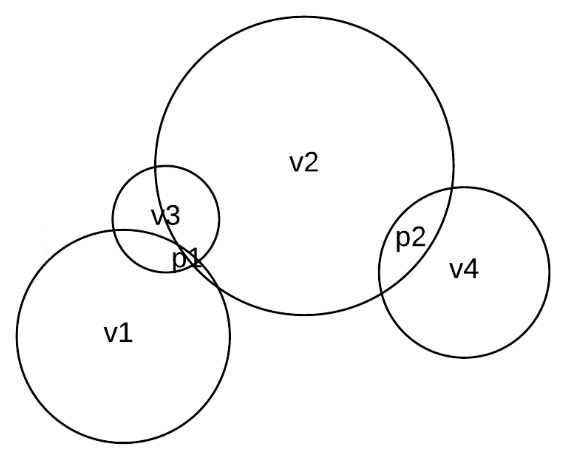
\includegraphics[scale=0.3]{images/exemple_introductif1.png}
  \caption{Exemple de ruches de fournisseurs}
  \label{fig:exemple_introductif_1}
\end{figure}

Soit $V = \{v_1, v_2, v_3, v_4\}$ un ensemble de fournisseurs (cf. Figure \ref{fig:exemple_introductif_1}.\\
En appliquant l'opérateur cellule $\pi_{v \in V}$ sur les fournisseurs de $V$, ayant chacun un rayon maximal quelconque, on aura les ruches :
\begin{itemize}
  \item{$R_1 = \{p_1, \{v_1, v_2, v_3\}\}$}
  \item{$R_2 = \{p_2, \{v_2, v_4\}\}$}
\end{itemize}
On constante ainsi que le fournisseur $v_2$ appartient simultanément aux ruches $R_1$ et $R_2$.\\
Par ailleurs, chaque fournisseur possède des voisins tels que :
\begin{itemize}
  \item{$\texttt{Voisins}(v_1) = \{v_2, v_3\}$}
  \item{$\texttt{Voisins}(v_2) = \{v_1, v_3, v_4\}$}
  \item{$\texttt{Voisins}(v_3) = \{v_1, v_2\}$}
  \item{$\texttt{Voisins}(v_4) = \{v_2, v_4\}$}
\end{itemize}
\end{example}

\begin{example}
\begin{figure}
  \centering
  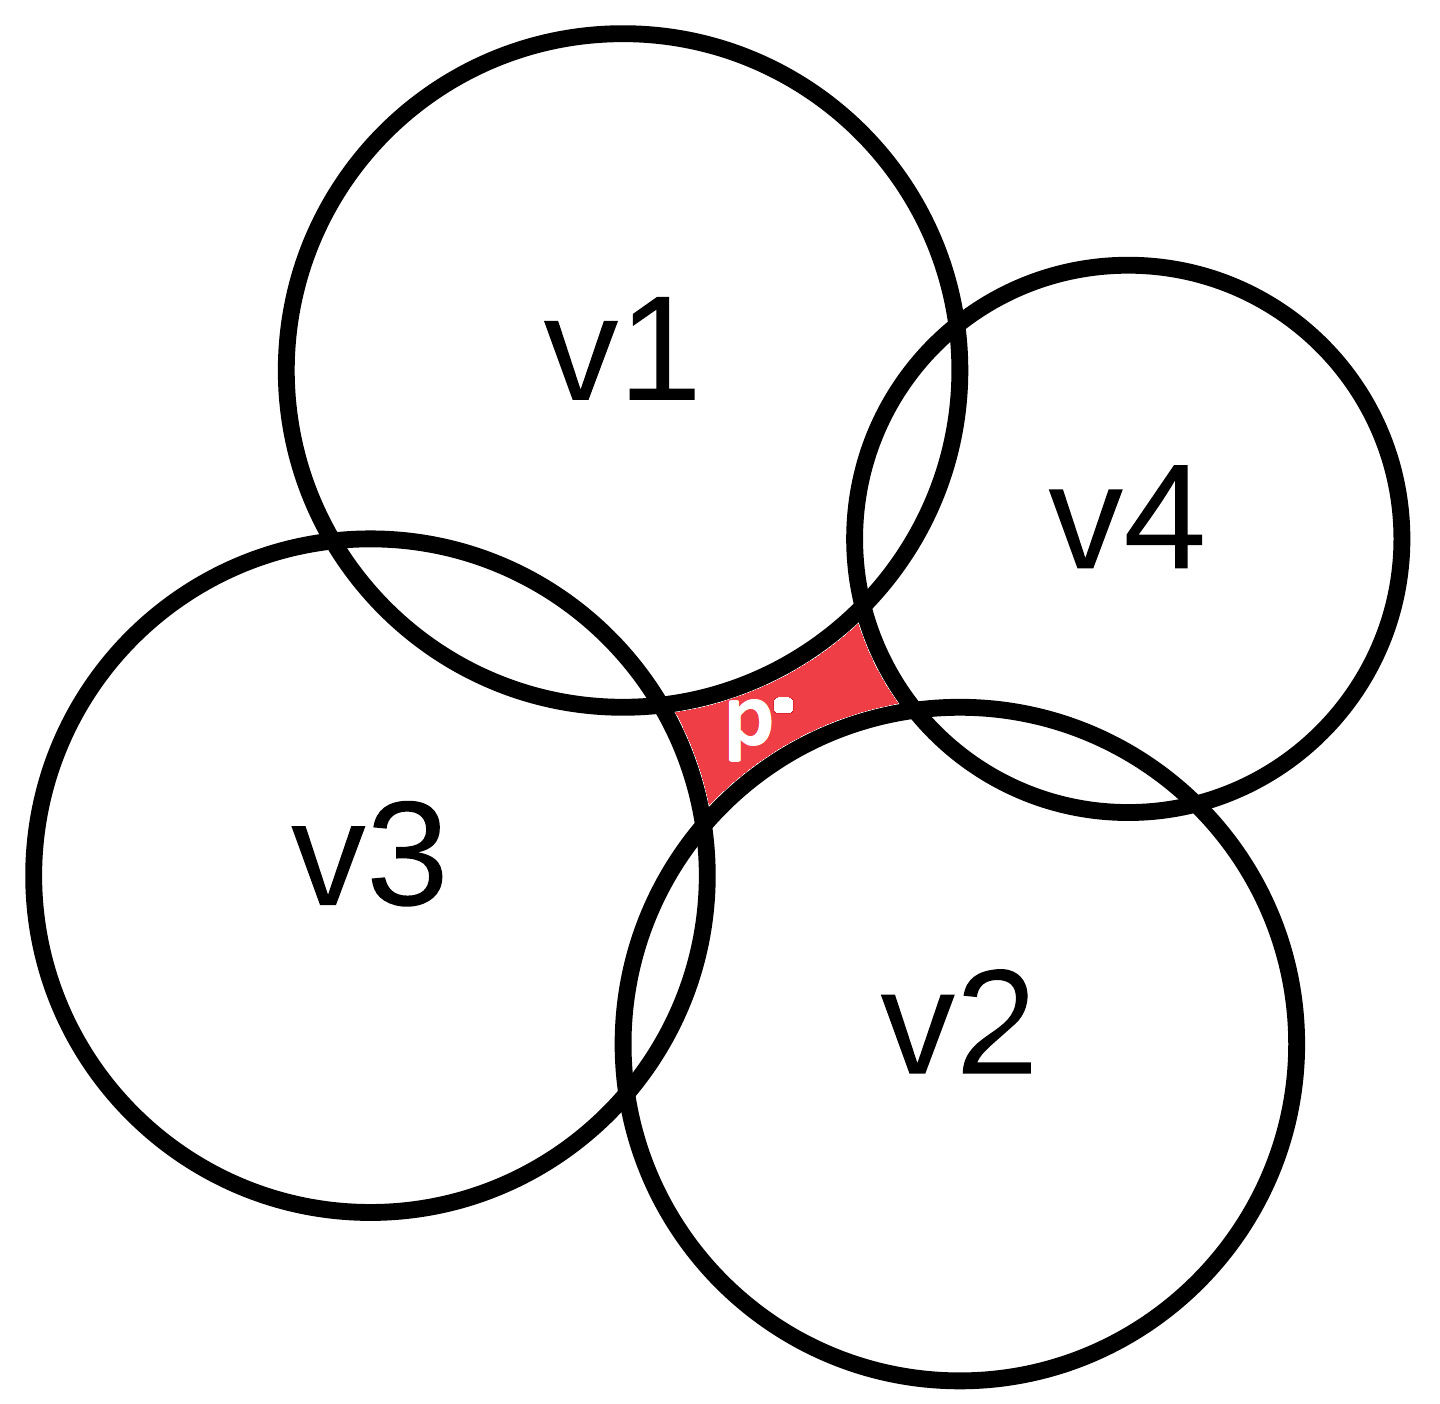
\includegraphics[scale=0.15]{images/exemple_introductif2.png}
  \caption{Exemple d'application du voisinage imposé sur des fournisseurs de ruches différentes}
  \label{fig:exemple_introductif_2}
\end{figure}

Soit $V = \{v_1, v_2, v_3, v_4\}$ un ensemble de fournisseurs (cf. Figure \ref{fig:exemple_introductif_2}.\\
En appliquant l'opérateur cellule $\pi_{v \in V}$ sur les fournisseurs de $V$, ayant chacun un rayon maximal quelconque, on aura les ruches :
\begin{itemize}
  \item{$R_1 = \{p_1, \{v_1, v_3\}\}$}
  \item{$R_2 = \{p_2, \{v_1, v_4\}\}$}
  \item{$R_3 = \{p_3, \{v_2, v_3\}\}$}
  \item{$R_4 = \{p_4, \{v_2, v_4\}\}$}
\end{itemize}
En appliquant la règle du \textit{voisinage imposé} sur les fournisseurs de $V$, on constate qu'il existe une ruche $R=\{p, \{v_1, v_2, v_3, v_4\}\}$ plus optimale les regroupant.
\end{example}

\subsubsection{remarques}
Les définitions dessus forment la base de notre approche d'optimisation. Il faut noter que d'autres propriétés et règles\footnote{amenant à la rédaction d'algorithmes d'optimisation} seront établies selon plusieurs cas d'usages qu'on étudiera lors de l'établissement de la version initiale\footnote{permettant de générer plus de cas à analyser avec plus de facilité, étant donné un support visuel} du site mais aussi lors des prochaines versions du site.

D'autre part, cette modélisation basée sur des \textbf{critères physiques} (\textit{rayon de déplacement maximal et coordonnées géographiques}) n'est pas suffisante pour couvrir l'ensemble des cas de formation de ruches. Ainsi en accord avec la philosophie de \textbf{XP}, lors de l'implémentation des prochaines versions, une \textbf{couche basée sur des critères logiques} (\textit{types de produits}) sera implémentée dessus pour étendre les possibilités du site face aux besoins croissants du marché.
%----------------------------------------------------------------------------------------
%   MODÈLE EA
%----------------------------------------------------------------------------------------
\section{Modèle EA}
\begin{figure}[!ht]
  \centering
  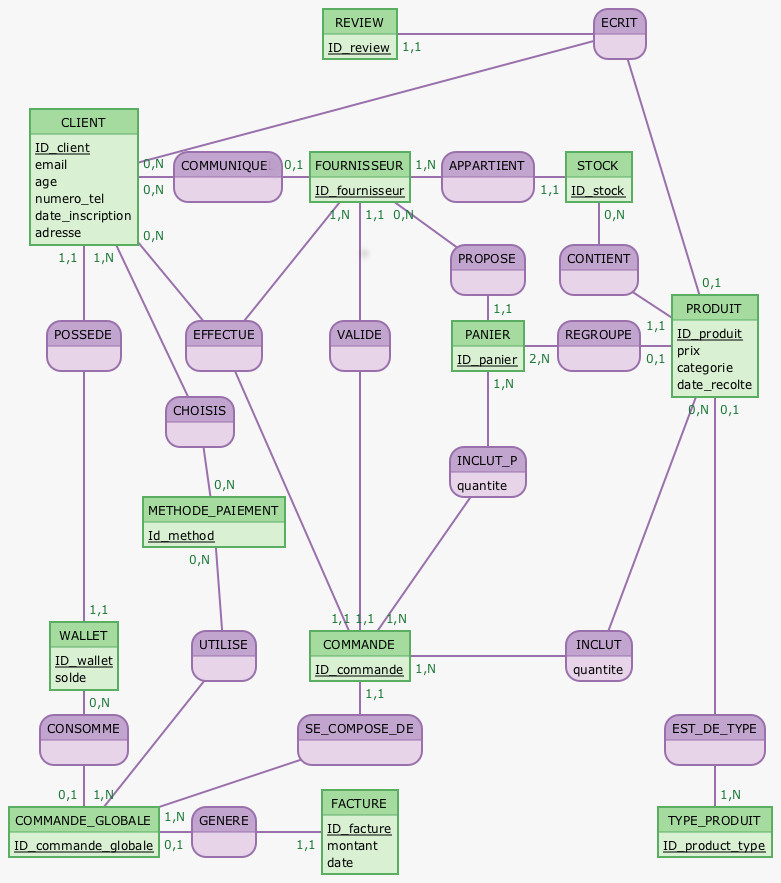
\includegraphics[scale=0.6]{images/Clients.jpg}
  \caption{Modèle Entité-Association}
  \label{fig:modele_EA}
\end{figure}

\newpage
%----------------------------------------------------------------------------------------
%   SCHÉMA DE BD
%----------------------------------------------------------------------------------------
\section{Schéma de base de données}
Le modèle relationnel obtenu par traduction du \textbf{modèle EA} des données est le suivant :
\begin{enumerate}
  \item { \texttt{REVIEW } (\underline{ID\_review}, \texit{ID\_client}, \texit{ID\_produit}) }
  \item { \texttt{CLIENT } (\underline{ID\_client}, \attr{email}, \attr{age}, \attr{numero\_tel}, \attr{date\_inscription}, \attr{adresse}) }
  \item { \texttt{FOURNISSEUR } (\underline{ID\_fournisseur}, \texit{ID\_commande}, \texit{ID\_client}) }
  \item { \texttt{STOCK } (\underline{ID\_stock}, \texit{ID\_fournisseur}) }
  \item { \texttt{PANIER } (\underline{ID\_panier}, \texit{ID\_fournisseur}) }
  \item { \texttt{PRODUIT } (\underline{ID\_produit}, \attr{prix}, \attr{categorie}, \attr{date\_recolte}, \texit{ID\_stock}, \texit{ID\_panier}, \texit{ID\_product\_type}) }
  \item { \texttt{CHOISIS } (\texit{\underline{ID\_client}}, \texit{\underline{Id\_method}}) }
  \item { \texttt{INCLUT\_P } (\texit{\underline{ID\_commande}}, \texit{\underline{ID\_panier}}, \attr{quantite}) }
  \item { \texttt{METHODE\_PAIEMENT } (\underline{Id\_method}) }
  \item { \texttt{WALLET } (\underline{ID\_wallet}, \attr{solde}, \texit{ID\_client}) }
  \item { \texttt{UTILISE } (\texit{\underline{ID\_commande\_globale}}, \texit{\underline{Id\_method}}) }
  \item { \texttt{COMMANDE } (\underline{ID\_commande}, \texit{ID\_commande\_globale}, \texit{ID\_client}, \texit{ID\_fournisseur}) }
  \item { \texttt{INCLUT } (\texit{\underline{ID\_commande}}, \texit{\underline{ID\_produit}}, \attr{quantite}) }
  \item { \texttt{COMMANDE\_GLOBALE } (\underline{ID\_commande\_globale}, \texit{ID\_wallet}) }
  \item { \texttt{FACTURE } (\underline{ID\_facture}, \attr{montant}, \attr{date}, \texit{ID\_commande\_globale}) }
  \item { \texttt{TYPE\_PRODUIT } (\underline{ID\_product\_type})}
\end{enumerate}
%----------------------------------------------------------------------------------------
%   CONCLUSION
%----------------------------------------------------------------------------------------
\chapter{Conclusion}
%----------------------------------------------------------------------------------------
%   IMPLÉMENTATION PRÉVUE
%----------------------------------------------------------------------------------------
\section{Implémentation prévue}
Pour la mise en oeuvre du site web, on prévoit utiliser, à part \textbf{HTML} et \textbf{CSS}, les outils suivants :
\begin{enumerate}
  \item{\textbf{JavaScript} et des \textbf{\textit{frameworks} pertinents} tels que \textbf{JQuery} et \textbf{Angular}, utilisés pour le développement \textit{front-end} du site web.}
  \item{le \textbf{\textit{framework} Bootstrap} pour faire des pages responsives adaptables aux dispositifs tels que smartphones, tablets, laptops et grand écrans.}
  \item{\textbf{MySQL} pour gérer la base de données du site : on a opté pour une base de données relationnelle vu le grand nombre d'associations reliant les différentes entités du site.}
  \item{\textbf{PHP} : suite au choix de \textbf{MySQL}, \textbf{PHP} (ainsi que les \textbf{\textit{frameworks}} basés dessus et \textbf{ORM}) est l'un des langages côté serveur les plus adaptés et les plus utilisés pour la manipulation d'un SGBD relationnel.}
\end{enumerate}

\begin{remark}
L'utilisation des \textbf{API} est aussi contemplée, notamment pour l'implémentation d'une carte (\textbf{Leaflet}), d'un chat securisé (\textbf{Telegram}), des méthodes de paiement, \textit{etc...}
\end{remark}
%----------------------------------------------------------------------------------------
%   PERSPECTIVES
%----------------------------------------------------------------------------------------
\section{Perspectives}
\label{sec:perspectives}
En plus des fonctionnalités que nous avons jugées être essentielles au projet et que nous prévoyons donc d'implémenter, nous avons pensé à des fonctionnalités supplémentaires que nous pourrions ajouter à notre projet une fois celles de base établies. En effet, plusieurs extensions sont possibles afin de proposer aux utilisateurs du site un choix plus diversifié.

Parmi celles-ci nous avons pensé au fait de proposer aux clients réalisant des achats sur le site d'avoir la possibilité de régler, en plus qu'avec un paiement bancaire, de pouvoir recourir à des services de paiements en ligne telles que Paypal, voire même d'offrir la possibilité de payer en Crypto-monnaie dans une version plus développée du projet.

En plus, nous pourrions également proposer plusieurs versions de notre site, où chaque version concerne un pays particulier et donc dans une langue précise. Tout cela, dans le but de pouvoir déployer le site ainsi que son concept à l'international.

D'autre part, nous avons formulé quelques \textit{user-stories} décrivant des fonctionnalités supplémentaires que nous souhaiterons ajouter aux prochaines versions du site, une fois la version de base établie et finalisée. Nous les expliciterons ainsi par la suite.
%----------------------------------------------------------------------------------------
%   USER-STORIES DE FONCTIONNALITÉ SUPPLÉMENTAIRES
%----------------------------------------------------------------------------------------
\subsection{\textit{User-Stories} des fonctionnalités supplémentaires}
\begin{userStory}[Création de Compte via des Plateformes Externes]
\textbf{En tant qu'utilisateur {\color{green}client}/{\color{red}fournisseur}}, je souhaite être capable de \textbf{créer un compte personnel via mon compte} \texttt{Facebook}/\texttt{Google},\\
\indent
\textbf{dans le but de} ne pas \textbf{remplir des formulaires} et \textbf{synchroniser mes données} entre les différentes plateformes hébergeant mes comptes personnels en ligne.
\end{userStory}

\begin{userStory}[Email Client $\leftrightarrows$ Fournisseur ou Fournisseur $\leftrightarrows$ Client/Fournisseur]
\textbf{En tant qu'utilisateur}, je souhaite communiquer avec d'autres \textbf{utilisateurs}\footnote{il n'y a pas d'emails entre deux utilisateurs {\color{green}clients}} (\textbf{{\color{green}client}} $\leftrightarrows$ \textbf{{\color{red}fournisseur}} ou \textbf{{\color{red}fournisseur}} $\leftrightarrows$ \textbf{{\color{green}client}/{\color{red}fournisseur}} via \textbf{email},\\
\indent
\textbf{dans le but d'}avoir une autre manière de les contacter \textbf{au plus tôt possible} au cas où il ne consulte pas régulièrement son compte utilisateur.
\end{userStory}

\begin{userStory}[Notifications sur les évenements de collecte]
\textbf{En tant qu'utilisateur {\color{green}client}/{\color{red}fournisseur}}, je souhaite \textbf{recevoir des notifications} sur les \textbf{événements de collecte à proximité}, que je soit participant aux événements ou pas,\\
\indent
\textbf{dans le but de} rester à jour par rapport aux \textbf{mouvements} des ruches à proximité.
\end{userStory}

\begin{userStory}[Date limite d'achat de produits]
\textbf{En tant qu'utilisateur {\color{red}fournisseur}}, je souhaite imposer des \textbf{dates limites d'achat} sur certains produits selon des conditions sur leurs quantités en stock,\\
\indent
\textbf{dans le but de personnaliser} mes \textbf{paramètres d'offre et demande} de produits tout en \textbf{traitant les commandes en cours}.
\end{userStory}

\begin{userStory}[Commandes retardées]
\textbf{En tant qu'utilisateur {\color{red}fournisseur}}, je souhaite offrir aux clients la chance d'effectuer des \textbf{commandes retardées} sur certains \textbf{produits en rupture de stock},\\
\indent
\textbf{dans le but de} garder mes portions du marché quand certains produits sont en rupture de stock.
\end{userStory}

\begin{userStory}[Méthodes de paiement]
\textbf{En tant qu'utilisateur {\color{green}client}}, je souhaite avoir des \textbf{méthodes de paiement sécurisées} à travers mon \textbf{compte bancaire}/\texttt{PayPal},\\
\indent
\textbf{dans le but de protéger mes identifiants financiers} et \textbf{compléter fiablement mes transactions}.
\end{userStory}

\begin{userStory}[Portefeuille virtuel]
\textbf{En tant qu'utilisateur {\color{green}client}}, je souhaite avoir un \textbf{portefeuille virtuel associé à mon compte utilisateur} et contenant des points de fidélité que je collecte à travers mon \textbf{activité sur le site},\\
\indent
\textbf{dans le but d'}avoir des \textbf{réductions} sur certains produits, définies par rapport aux \textbf{points de fidélité collectés}.
\end{userStory}

\begin{userStory}[Reçu]
\textbf{En tant qu'utilisateur {\color{green}client}/{\color{red}fournisseur}}, je souhaite recevoir un \textbf{reçu} à la fin de chaque \textbf{transaction} via \textbf{sms} et/ou \textbf{email}, tout en \textbf{mettant à jour l'historique de mes achats/ventes},\\
\indent
\textbf{dans le but de suivre l'historique de mes achats/ventes} à travers \textbf{différents médias} pour plus d'\textbf{accesibilité} et d'\textbf{intégrité}.
\end{userStory}

\begin{userStory}[Purchase Cancellation \} Reimbursment Policy]
\textbf{En tant qu'utilisateur {\color{green}client}}, je souhaite avoir la possibilité d'\textbf{annuler un achat} dans un \textbf{délai spécifique} suivant la transaction,\\
\indent
\textbf{dans le but d'}être \textbf{remboursé partiellement/complétement} suite à la transaction défectueuse.
\end{userStory}

\begin{figure}[!ht]
  \centering
  \begin{tikzpicture}
    \setcounter{tikzumlUseCaseNum}{0}
    \umlactor[x=-2]{Client}
    \umlactor[x=-2, y=-4]{Database}
    \umlactor[x=11, y=-6.2]{Vendor User Database}
    \umlactor[x=11, y=-11]{Money Payment Platform}
    \umlactor[x=6, y=-14]{Bill Reception Platform}
    \umlactor[x=1, y=-14]{Bank/PayPal}
    \begin{umlsystem}[x=1, fill=green!10]{client home page}
      \umlusecase[width=2cm] {Add Items to Shopping Cart} %1
      \umlusecase[x=5, width=2cm]{Delete Items from Shopping Cart} %2
      \umlusecase[x=2, y=-3, width=3cm]{Choose Time of Collection} %3
      \umlusecase[x=5, y=-5, width=3cm]{Choose Payment Method} %4
      \umlusecase[x=5, y=-9, width=3cm]{Get Reductions from Wallet Points} %5
      \umlusecase[y=-12]{Check Wallet} %6
      \umlusecase[y=-9, width=3cm]{Checkout from Payment} %7
      \umlusecase[y=-5, width=3cm]{Update Purchases' History} %8
      \umlusecase[x=5, y=-12, width=3cm]{Receive Bill} %9
    \end{umlsystem}
    \begin{umlsystem}[x=11.2, fill=red!10]{vendor home page}
      \umlusecase[width=1.5cm]{Send a Bill} %10
    \end{umlsystem}
    \umlextend{usecase-2}{usecase-1}
    \umlextend{usecase-5}{usecase-4}
    \umlinclude{usecase-1}{usecase-3}
    \umlinclude{usecase-3}{usecase-4}
    \umlinclude{usecase-7}{usecase-8}
    \umlinclude[pos stereo=0.2]{usecase-9}{usecase-8}
    \umlassoc{Client}{usecase-1}
    \umlassoc{Client}{usecase-6}
    \umlassoc{Money Payment Platform}{usecase-4}
    \umlHVassoc{Money Payment Platform}{usecase-7}
    \umlassoc{Vendor User Database}{usecase-7}
    \umlassoc{Vendor User Database}{usecase-9}
    \umlassoc[name=send]{Vendor User Database}{usecase-10}
    \umlassoc{Bill Reception Platform}{usecase-9}
    \umlassoc{Bank/PayPal}{usecase-9}
    \umlassoc{Database}{usecase-8}
    \umlnote[x=9, y=-3]{usecase-10}{only if transaction validated by vendor}
  \end{tikzpicture}
  \caption{Diagramme de cas d'usage des fonctionnalités de la gestion des commandes et du paiement du point de vue du client}
  \label{fig:order_payment_client_use_case_diagram}
\end{figure}

\begin{figure}[!ht]
  \centering
  \begin{tikzpicture}
    \setcounter{tikzumlUseCaseNum}{0}
    \umlactor{Vendor}
    \umlactor[x=12, y=-2]{Database}
    \umlactor[y=-13]{Client User Database}
    \umlactor[x=12, y=-11]{Bill Reception Platform}
    \umlactor[x=4.5, y=-13]{Bank/PayPal}
    \begin{umlsystem}[x=4, fill=red!10]{vendor home page}
      \umlusecase[width=2cm]{Check Stocks}
      \umlusecase[x=5, width=2cm]{Allow Delayed Orders}
      \umlusecase[x=2.6, y=-3, width=3cm]{Set Purchase Deadline}
      \umlusecase[x=4, y=-6, width=3cm]{Check Pending Orders}
      \umlusecase[y=-8, width=2cm]{Process Pending Orders}
      \umlusecase[x=5, y=-8, width=2cm]{Send Bill}
      \umlusecase[x=4.5, y=-11, width=2cm]{Update Sales' History}
    \end{umlsystem}
    \umlextend{usecase-2}{usecase-1}
    \umlextend[name=deadline]{usecase-3}{usecase-4}
    \umlextend[name=checkPending1]{usecase-4}{usecase-5}
    \umlinclude{usecase-5}{usecase-6}
    \umlinclude{usecase-6}{usecase-7}
    \umlassoc{Vendor}{usecase-1}
    \umlassoc[name=checkPending2]{Vendor}{usecase-4}
    \umlassoc[name=process]{Vendor}{usecase-5}
    \umlassoc{Database}{usecase-2}
    \umlassoc{Database}{usecase-3}
    \umlassoc{Database}{usecase-4}
    \umlassoc{Database}{usecase-7}
    \umlassoc{Bill Reception Platform}{usecase-6}
    \umlassoc{Bank/PayPal}{usecase-6}
    \umlassoc{Client User Database}{usecase-6}
    \umlnote[x=-0.5, y=-5]{checkPending1-1}{only if validating transactions is set to manual}
    \umlnote[x=-0.5, y=-5]{checkPending2-1}{only if validating transactions is set to manual}
    \umlnote[x=-0.5, y=-8]{process-1}{only if validating transactions is set to automatic}
    \umlnote[x=-0.5, y=-11]{deadline-1}{according to the number of pending orders}
  \end{tikzpicture}
  \caption{Diagramme de cas d'usage des fonctionnalités de la gestion des commandes et du paiement du point de vue du fournisseur}
  \label{fig:order_payment_vendor_use_case_diagram}
\end{figure}
%----------------------------------------------------------------------------------------
%   ANNEXES
%----------------------------------------------------------------------------------------
\begin{appendices}
%----------------------------------------------------------------------------------------
%   STORYBOARD
%----------------------------------------------------------------------------------------
\chapter{Storyboard}
\label{app:storyoard}
Dans ce chapitre, on illustre ci-dessous un \textit{mockup} graphique permettant de décrire une \textbf{structure de mise en forme approximative}, ainsi qu'un \textbf{enchaînement d'évènements et de fonctionnalités} résultant d'une \textbf{navigation partielle} de notre site web.

\begin{figure}[!ht]
  \centering
  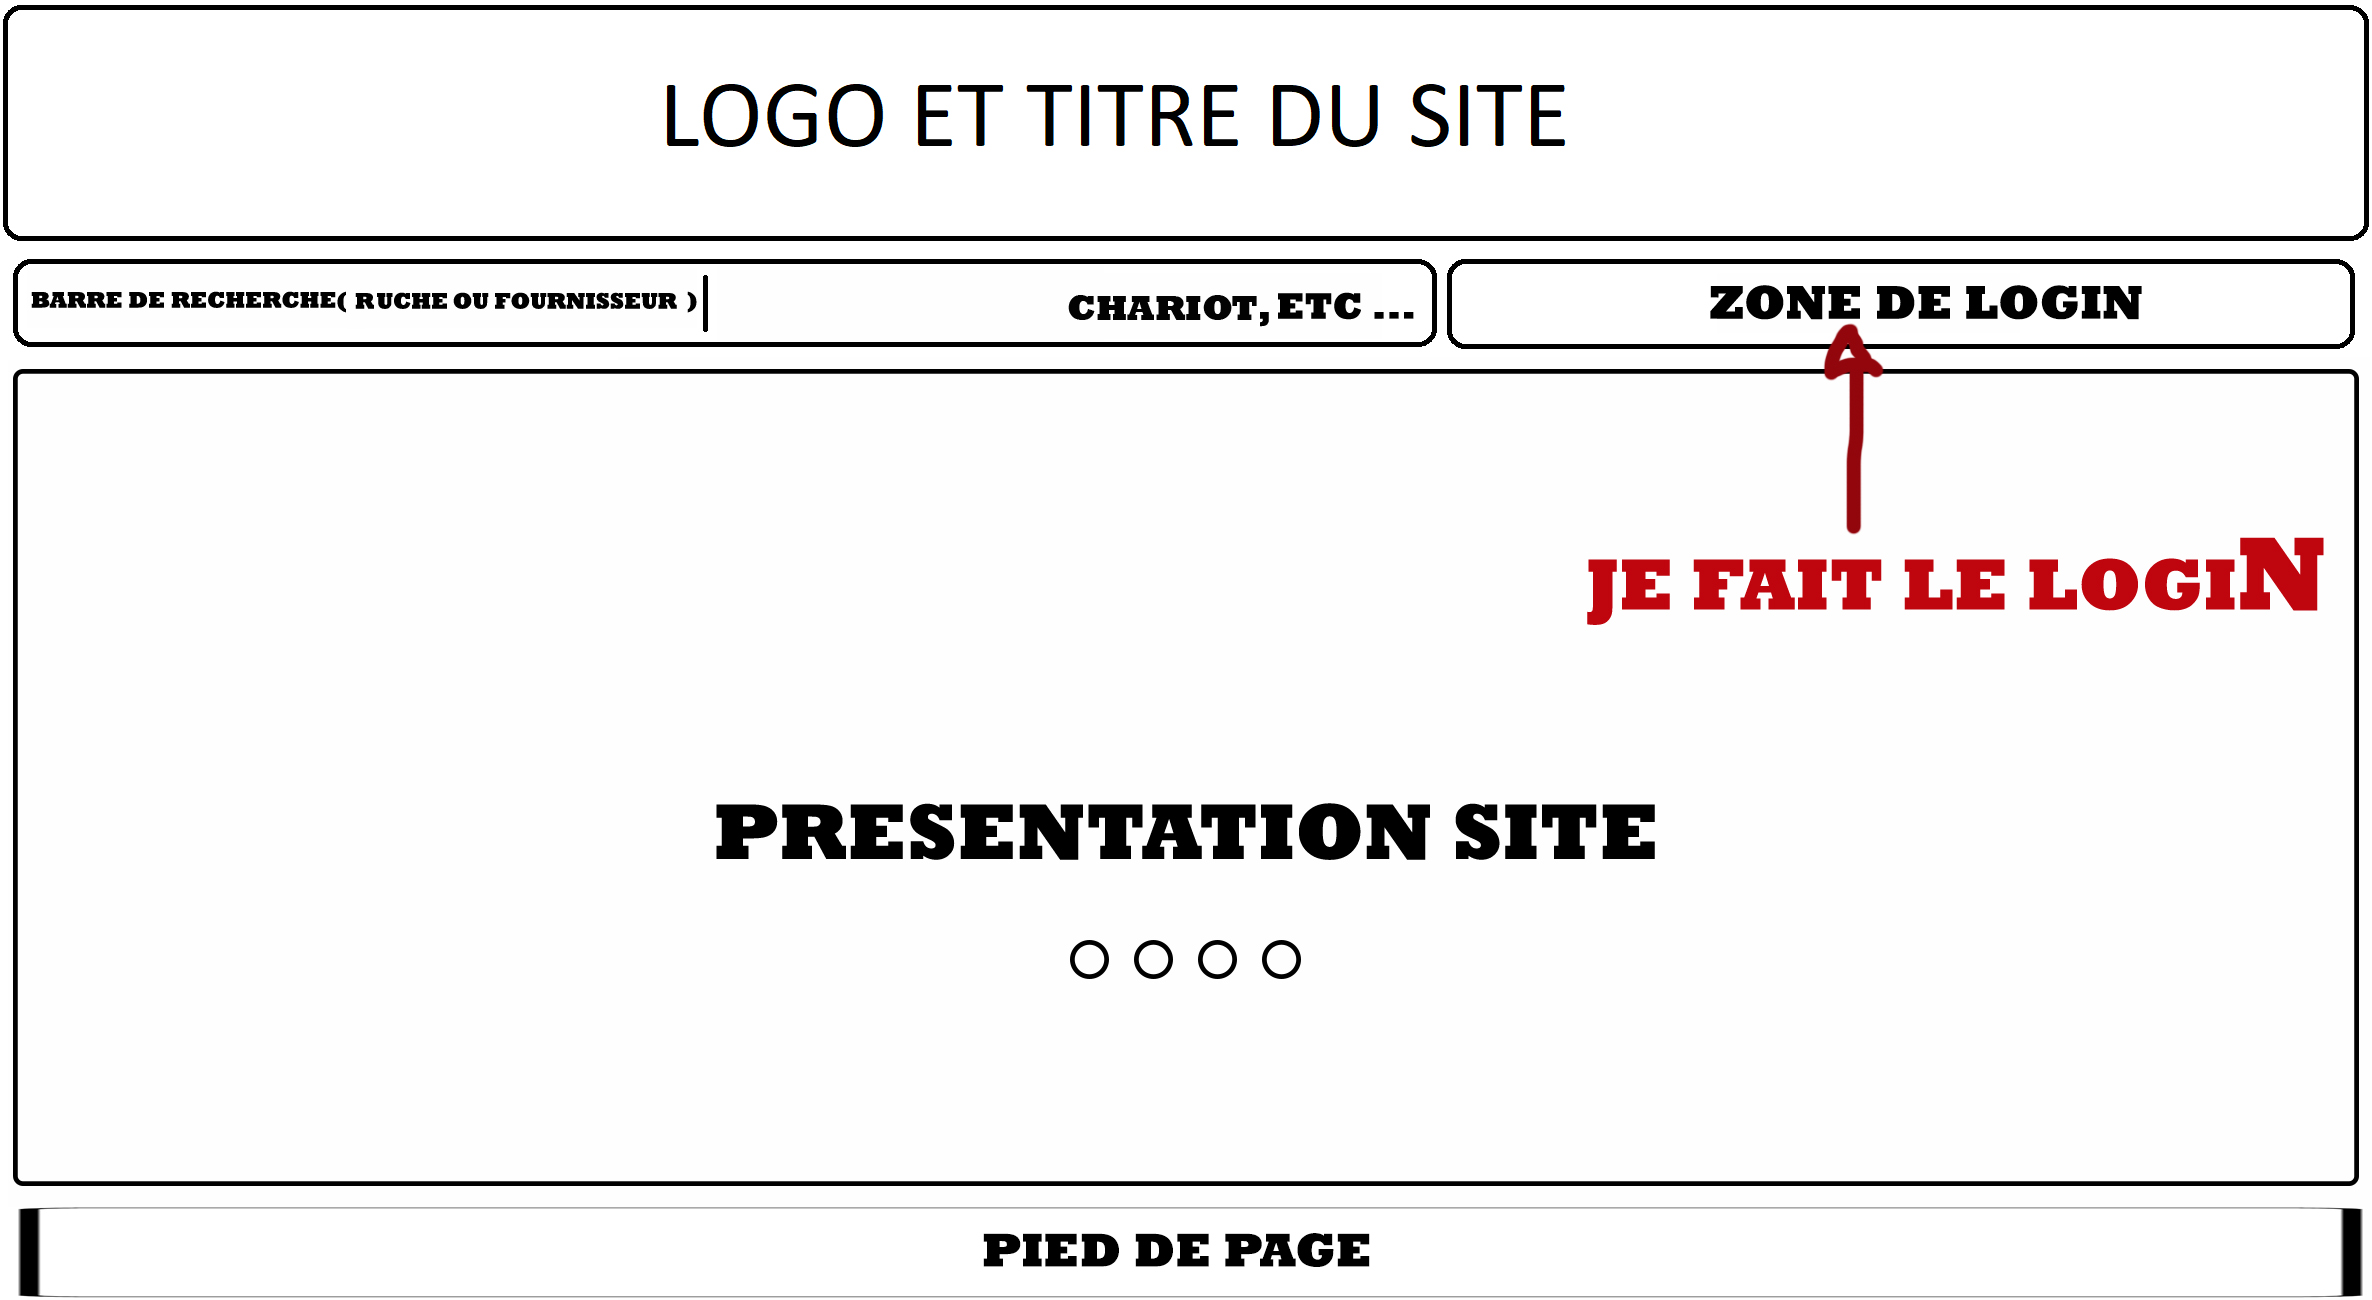
\includegraphics[scale=0.25]{images/storyboard/00.jpg}
  \caption{Page d'accueil et zone de login}
\end{figure}

\begin{figure}[!ht]
  \centering
  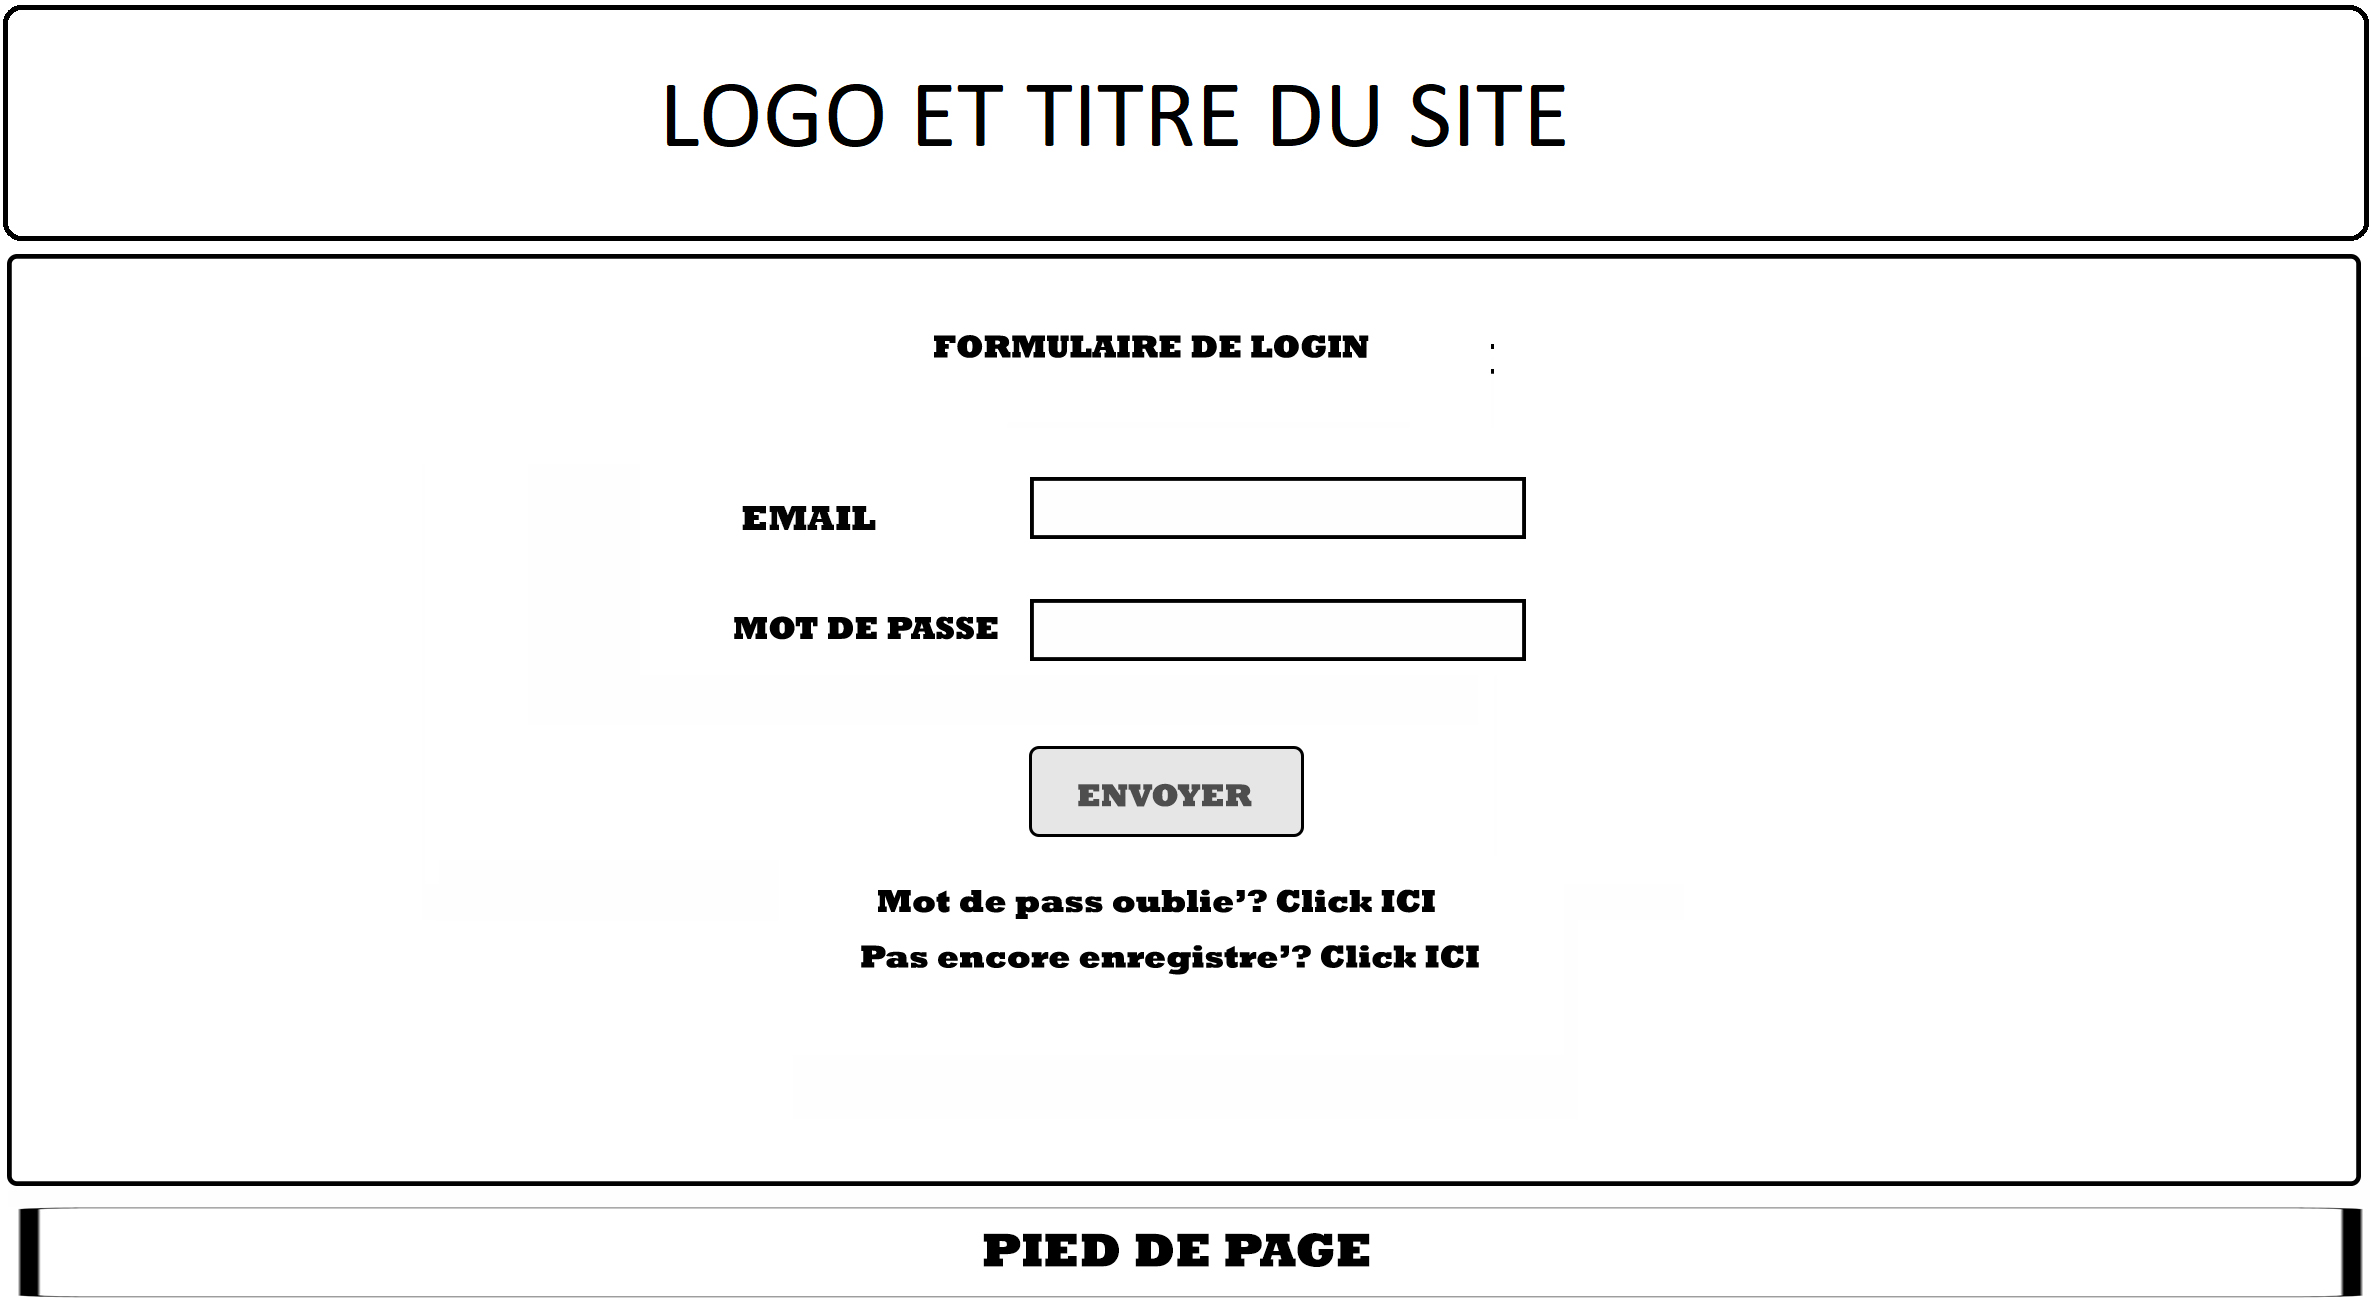
\includegraphics[scale=0.25]{images/storyboard/01.jpg}
  \caption{Page de login}
\end{figure}

\begin{figure}[!ht]
  \centering
  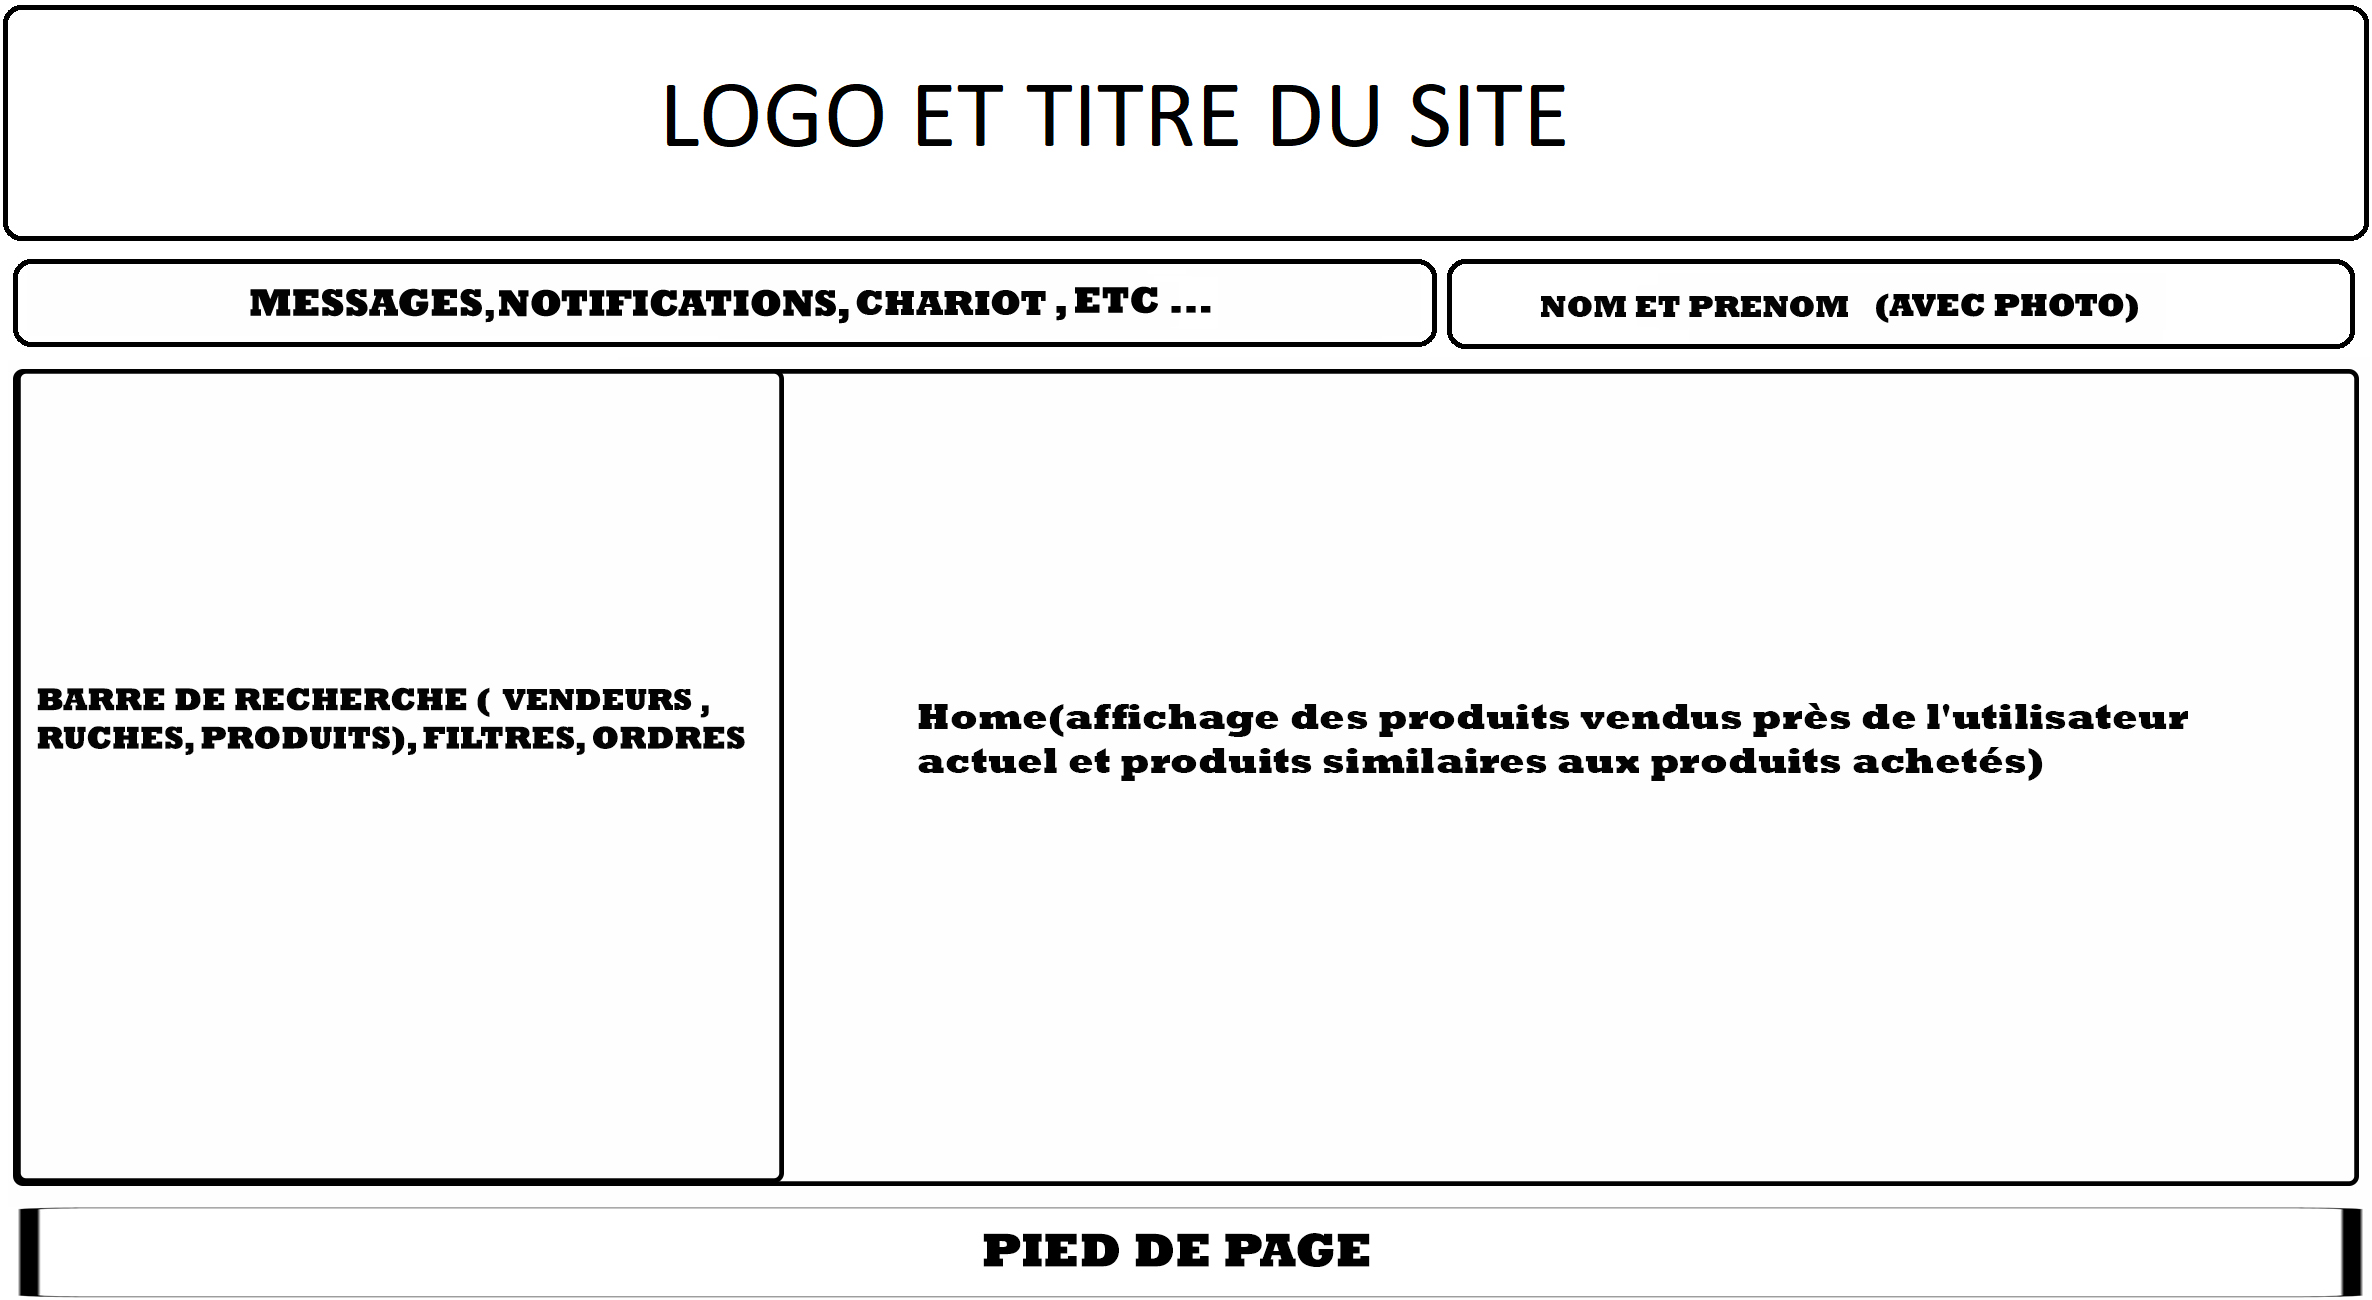
\includegraphics[scale=0.25]{images/storyboard/02.jpg}
  \caption{Page d'accueil de l'utilisateur}
\end{figure}

\begin{figure}[!ht]
  \centering
  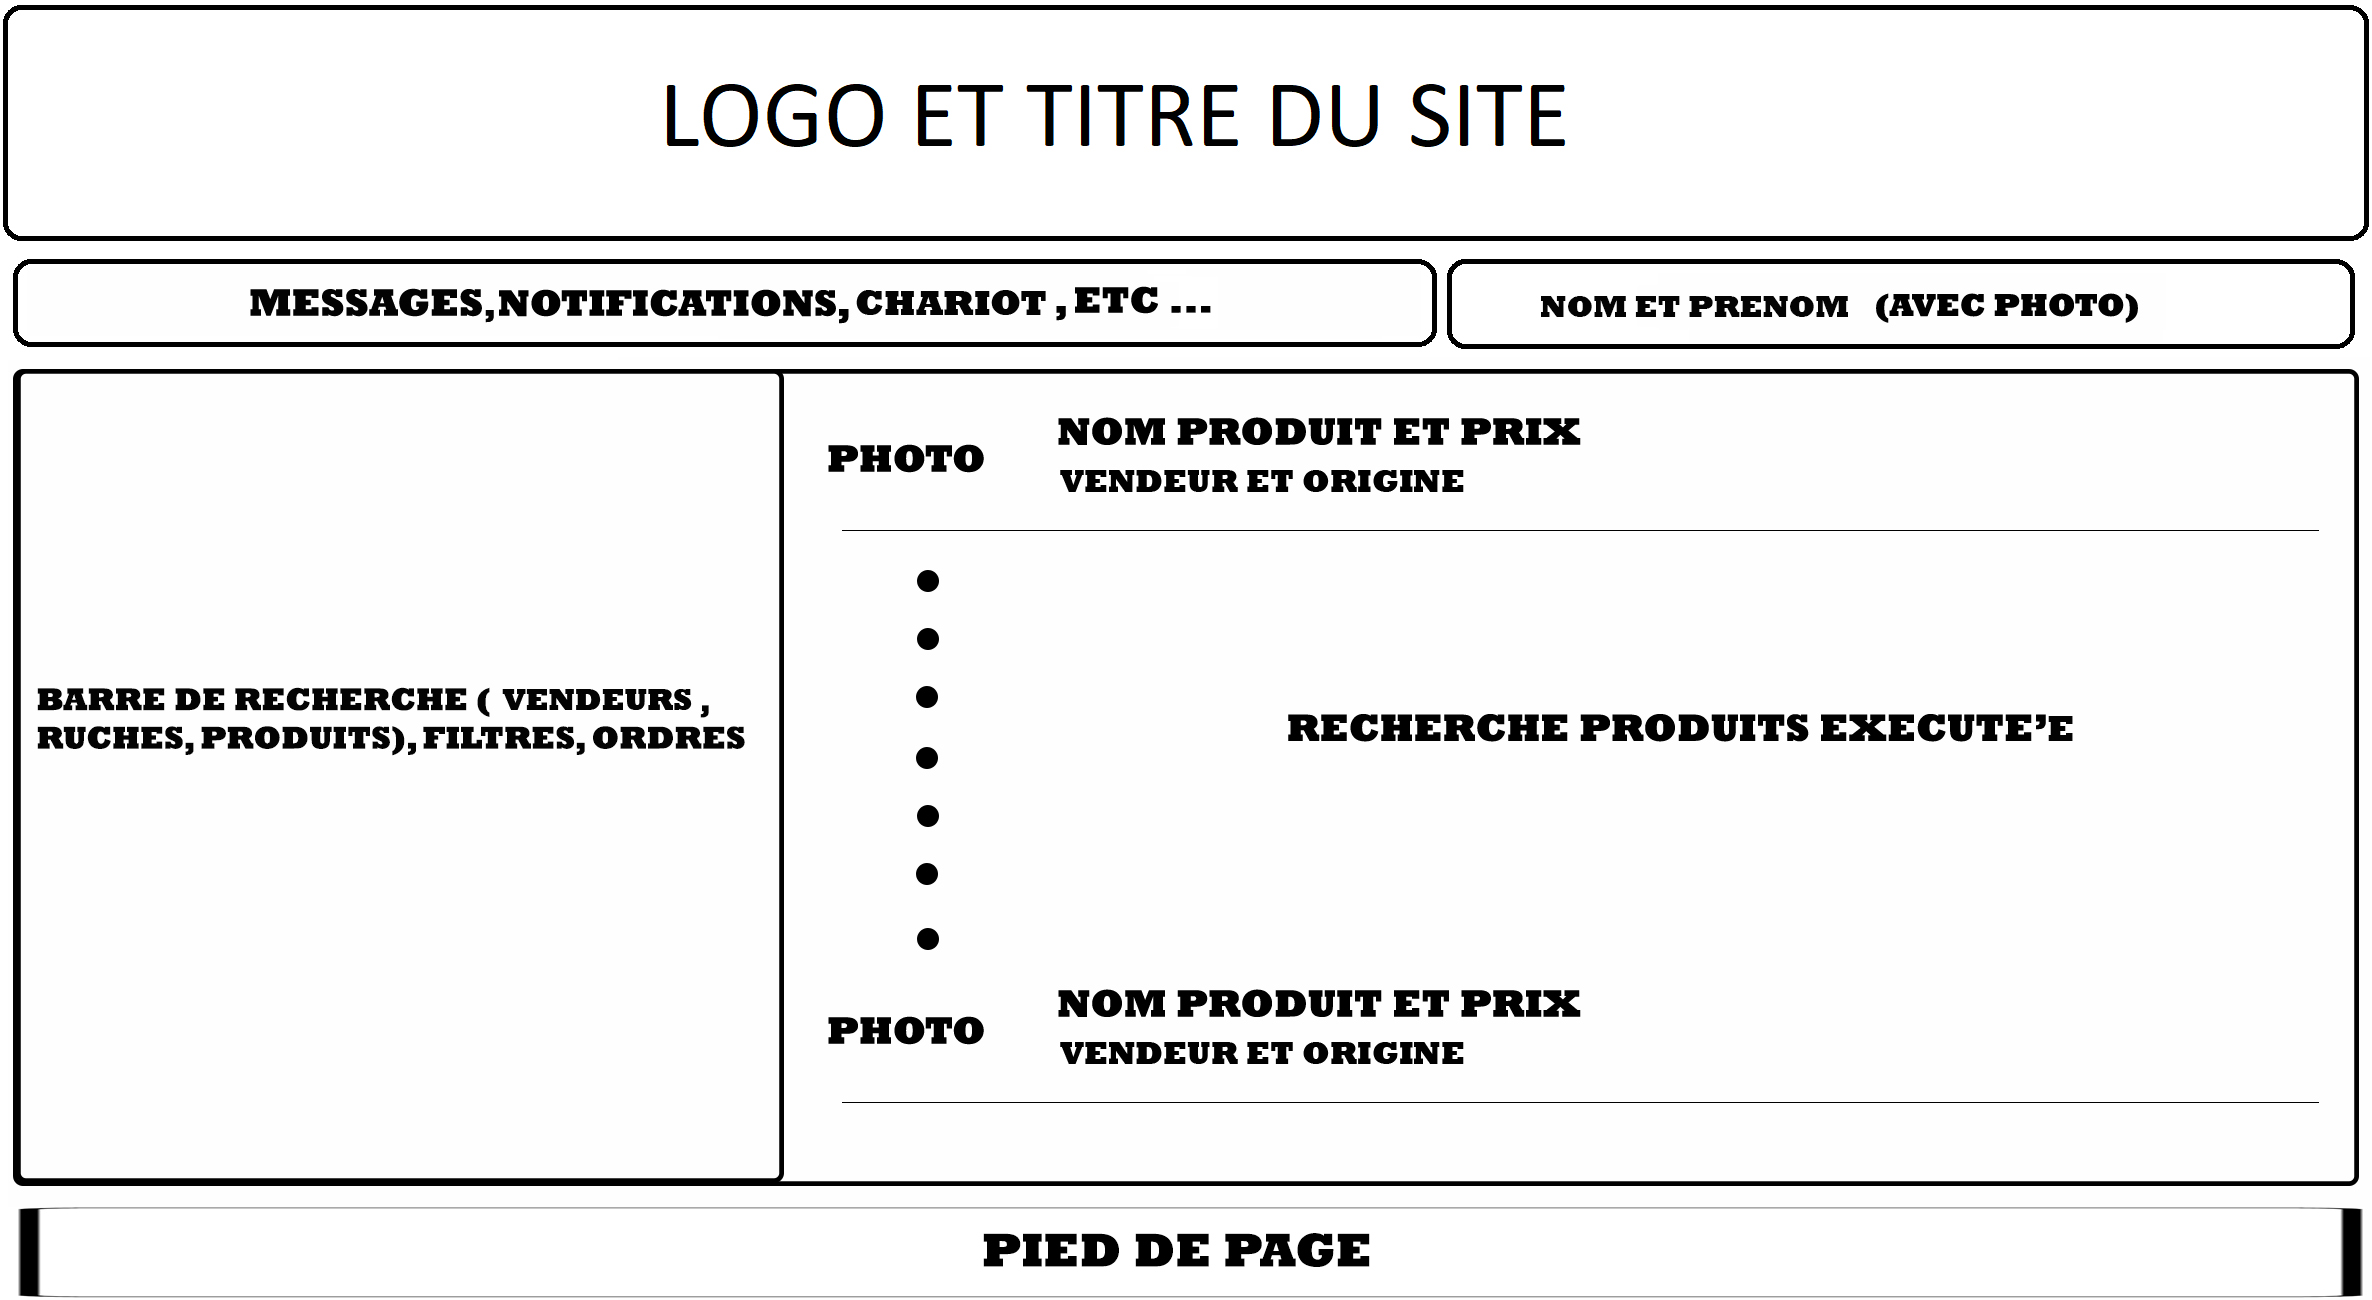
\includegraphics[scale=0.25]{images/storyboard/03.jpg}
  \caption{Recherche de produits}
\end{figure}

\begin{figure}[!ht]
  \centering
  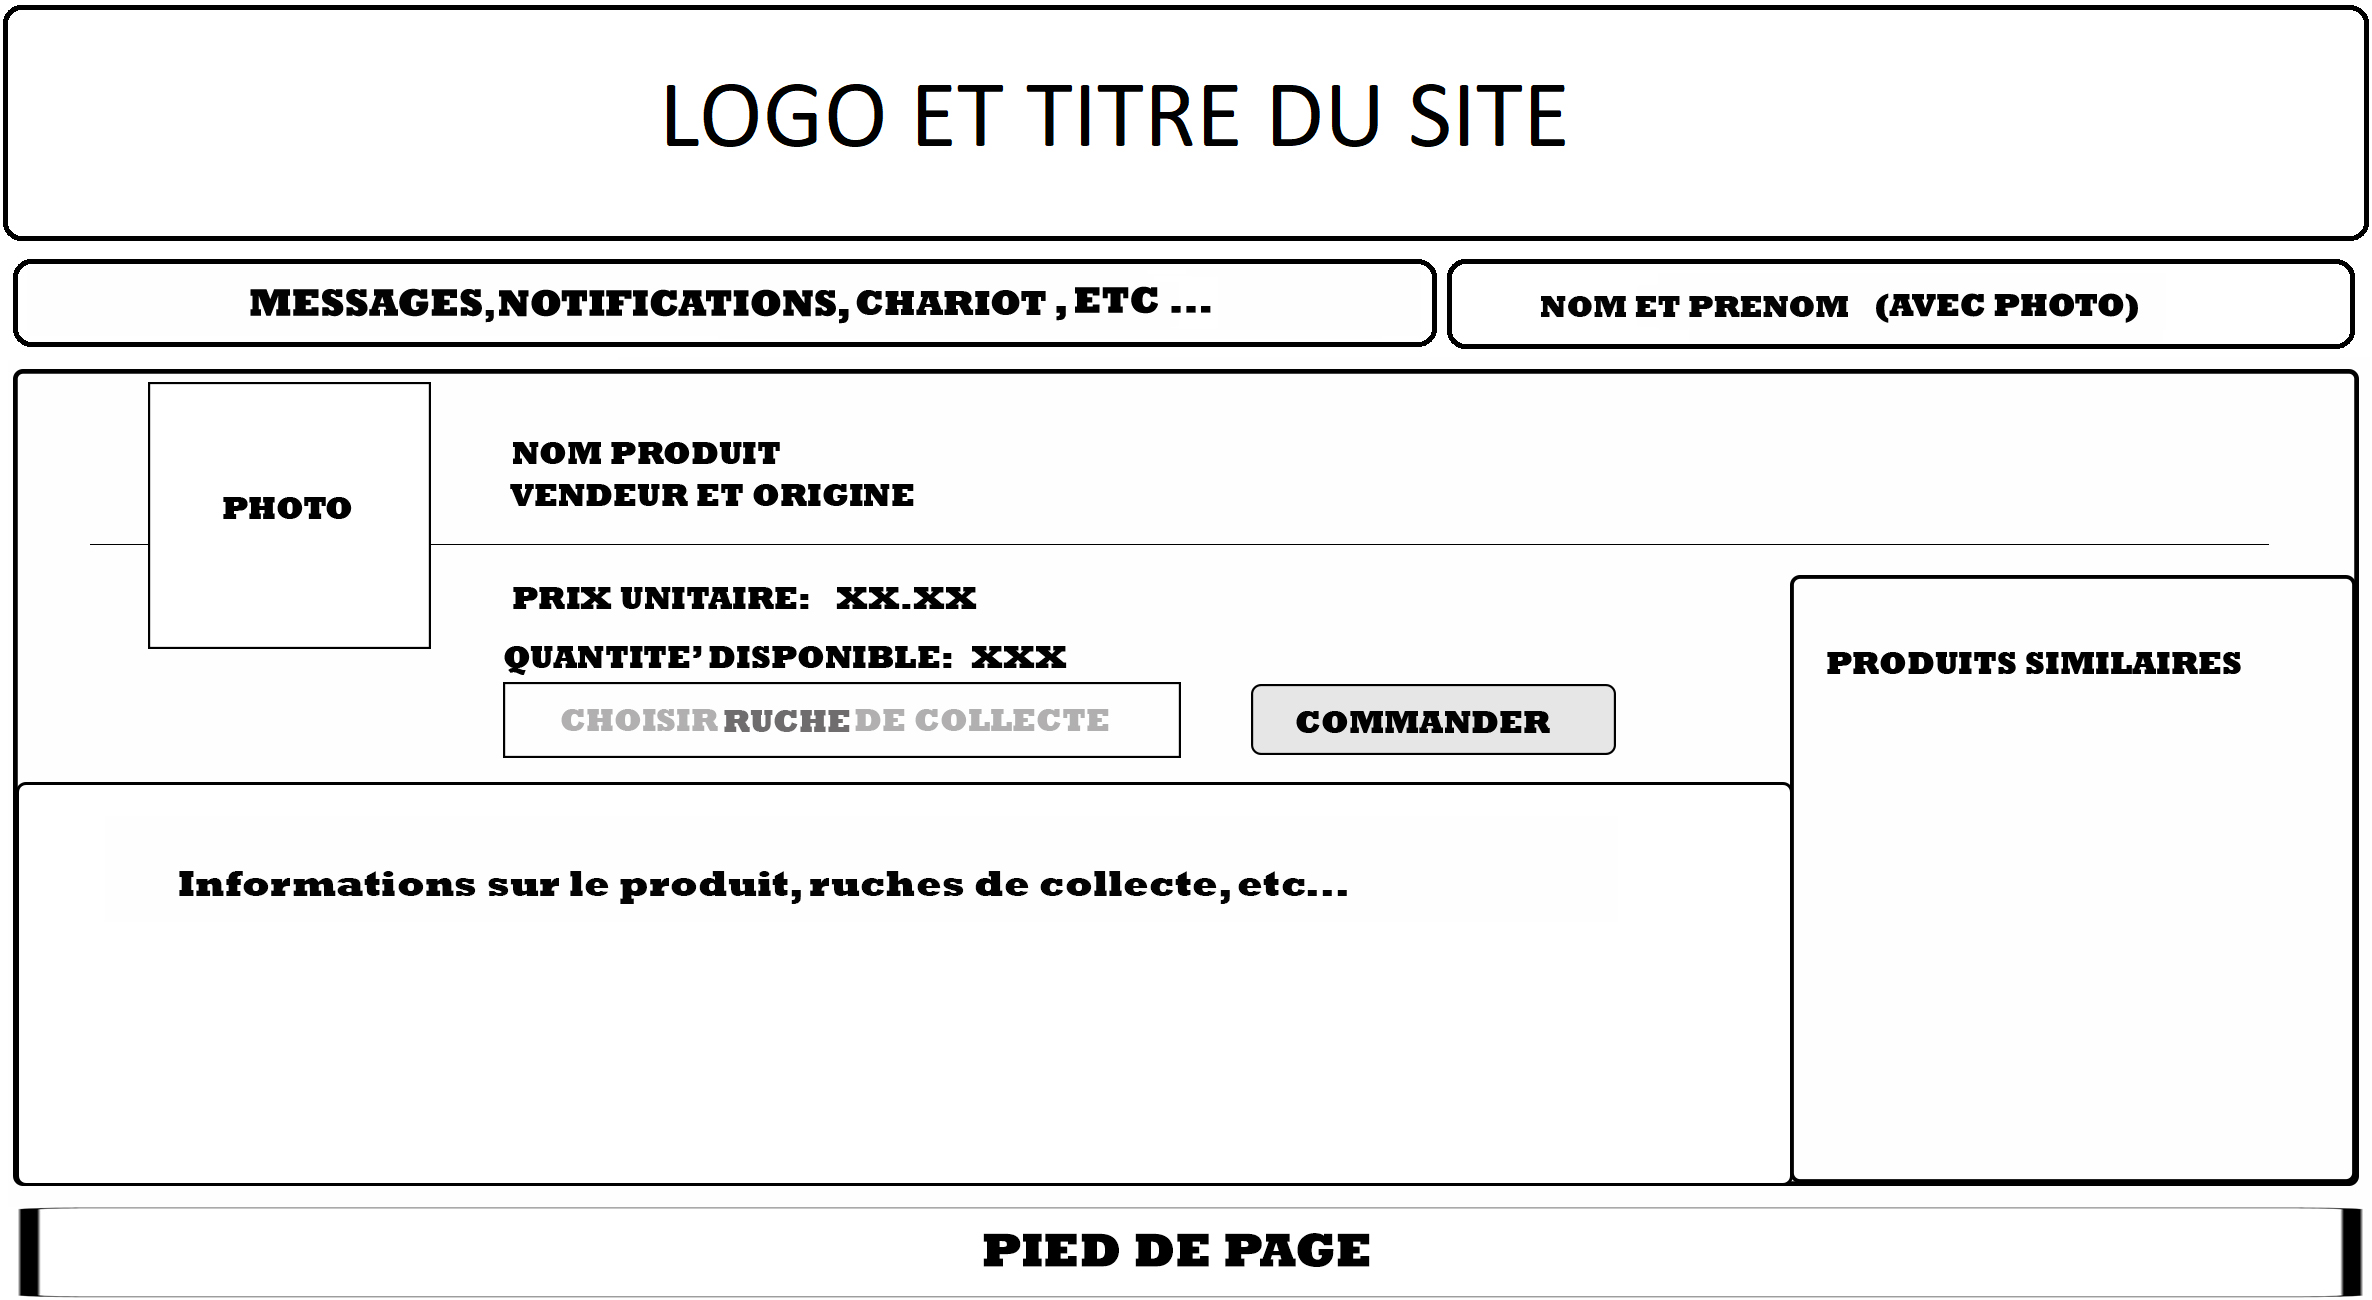
\includegraphics[scale=0.25]{images/storyboard/04.jpg}
  \caption{Informations sur un produit}
\end{figure}

\begin{figure}[!ht]
  \centering
  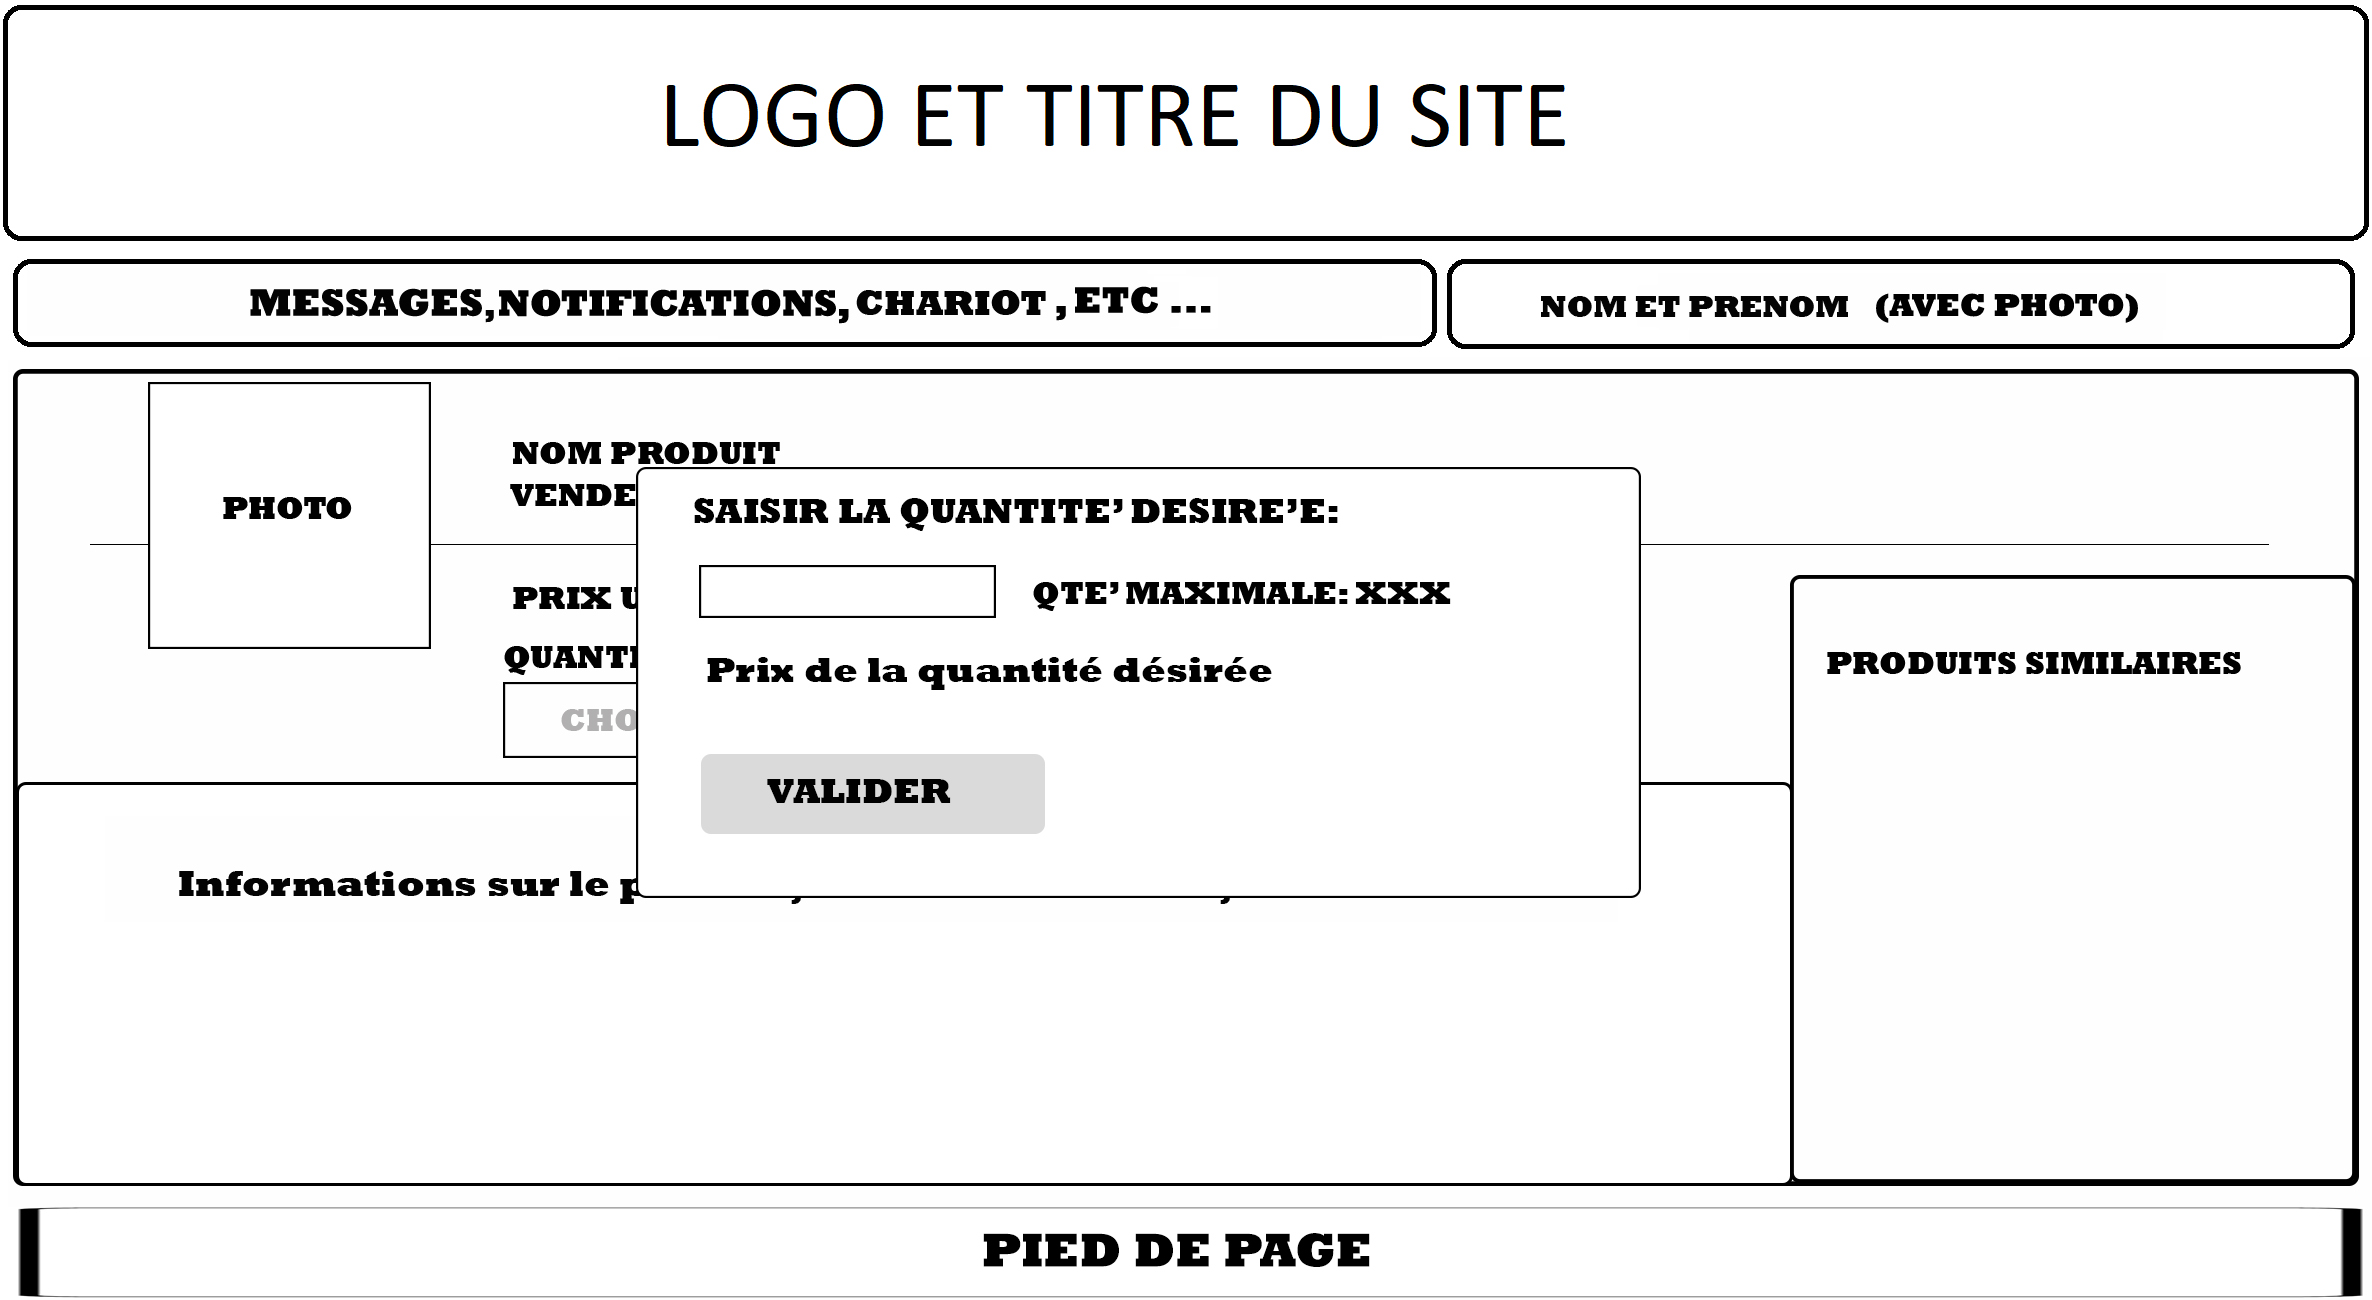
\includegraphics[scale=0.25]{images/storyboard/04_1.jpg}
  \caption{Commander un produit}
\end{figure}

\begin{figure}[!ht]
  \centering
  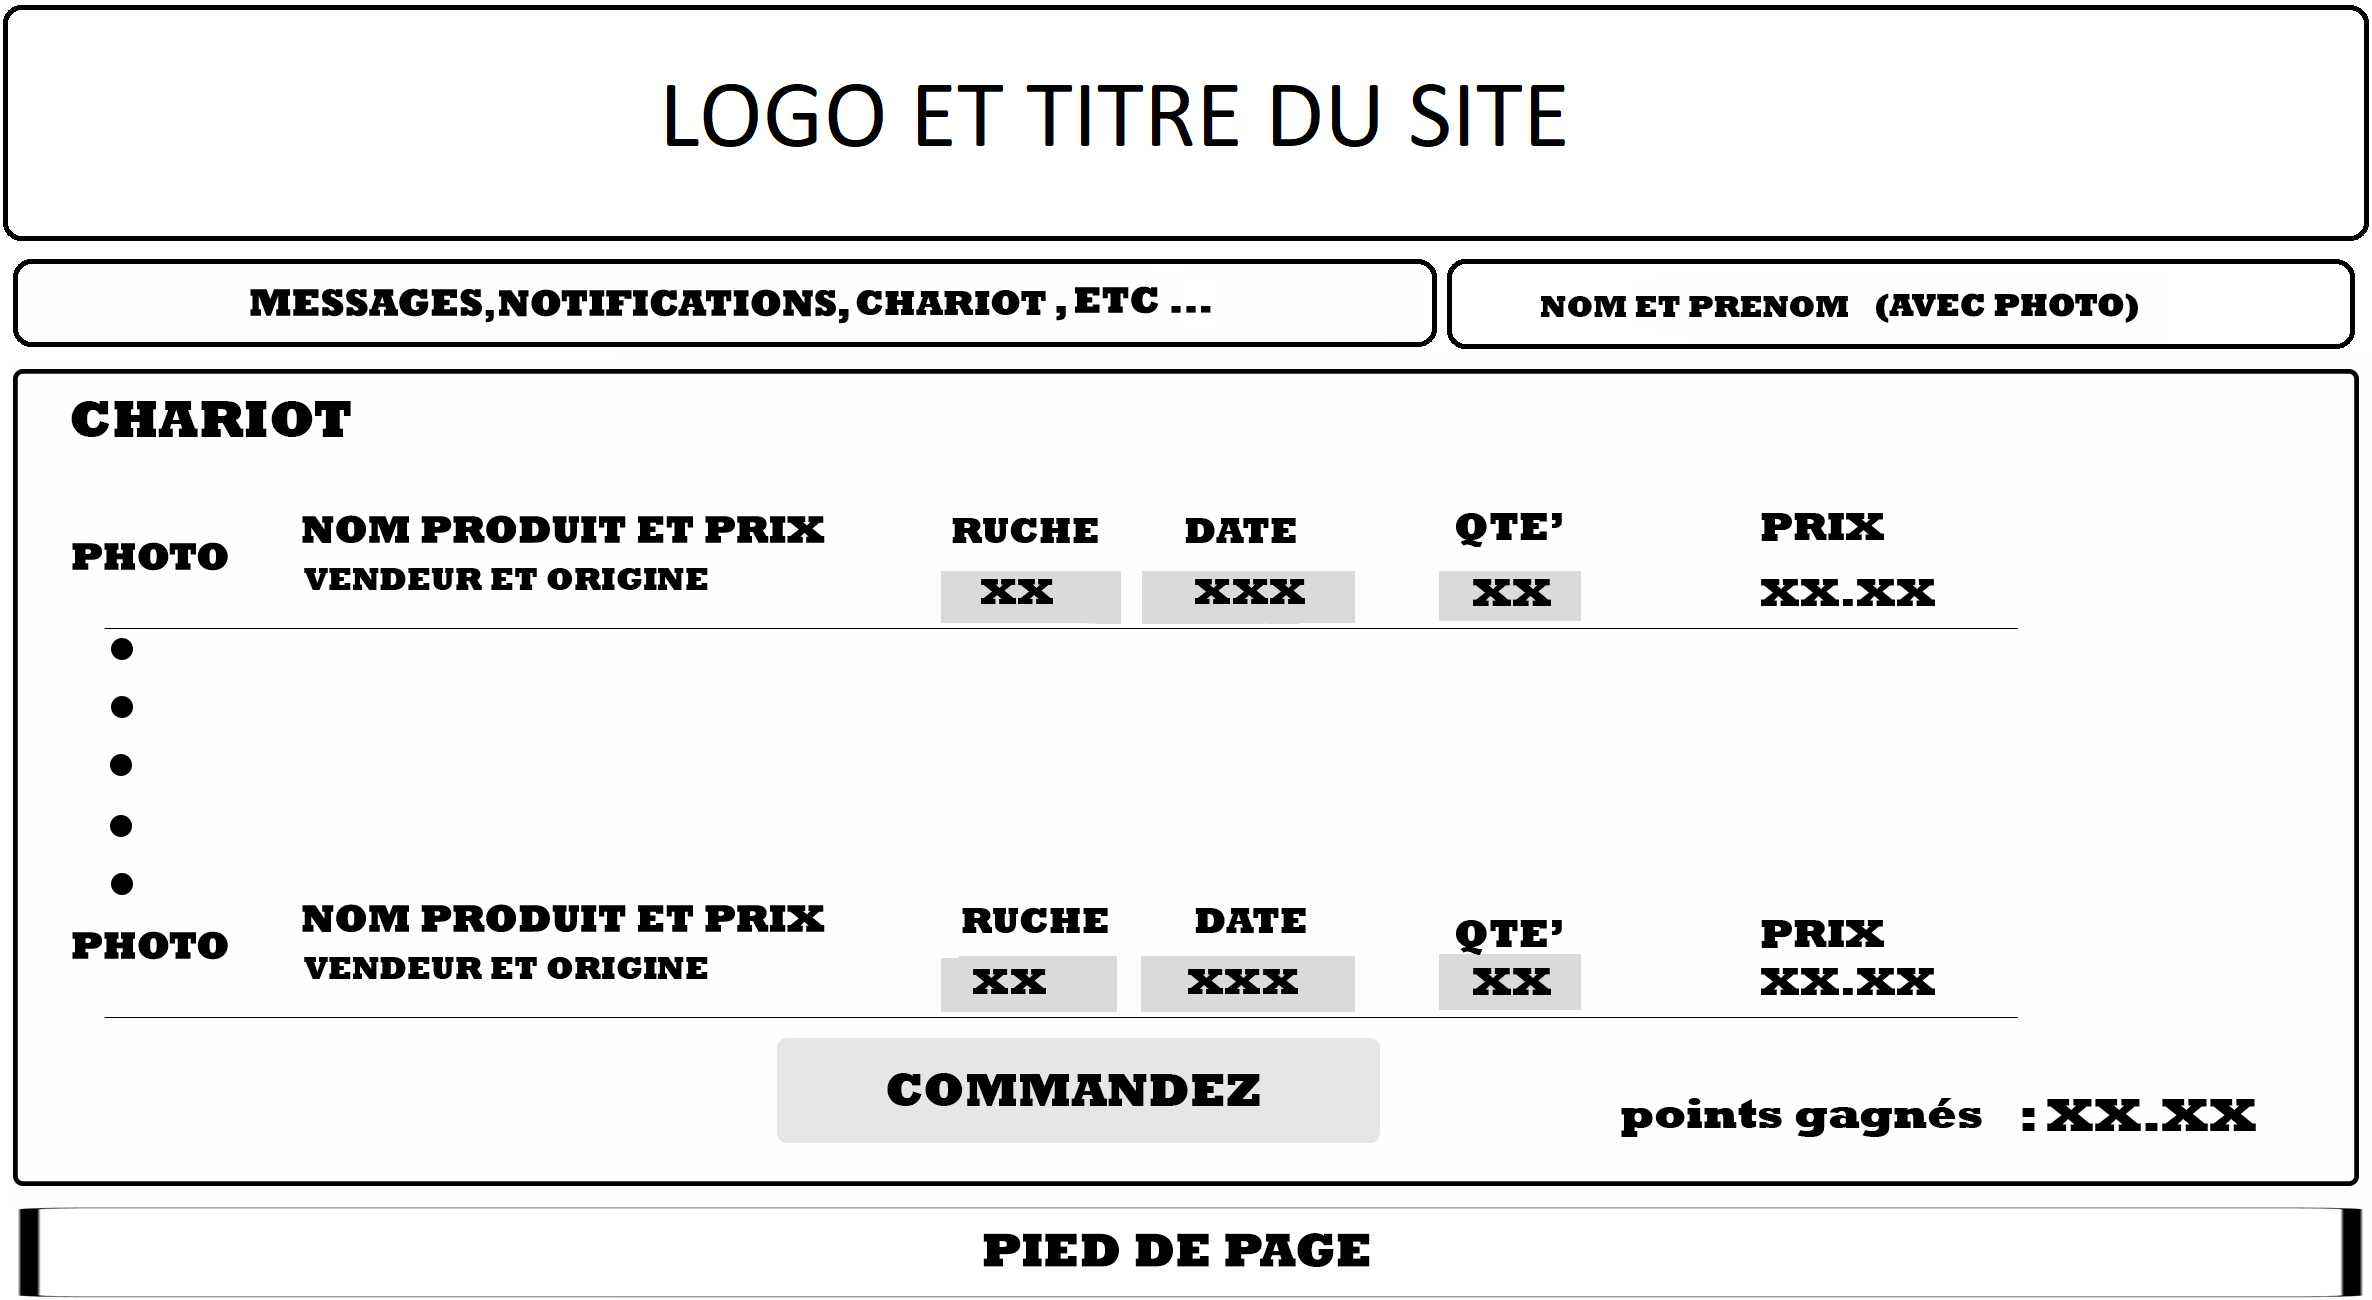
\includegraphics[scale=0.25]{images/storyboard/04_2.jpg}
  \caption{Chariot}
\end{figure}

\begin{figure}[!ht]
  \centering
  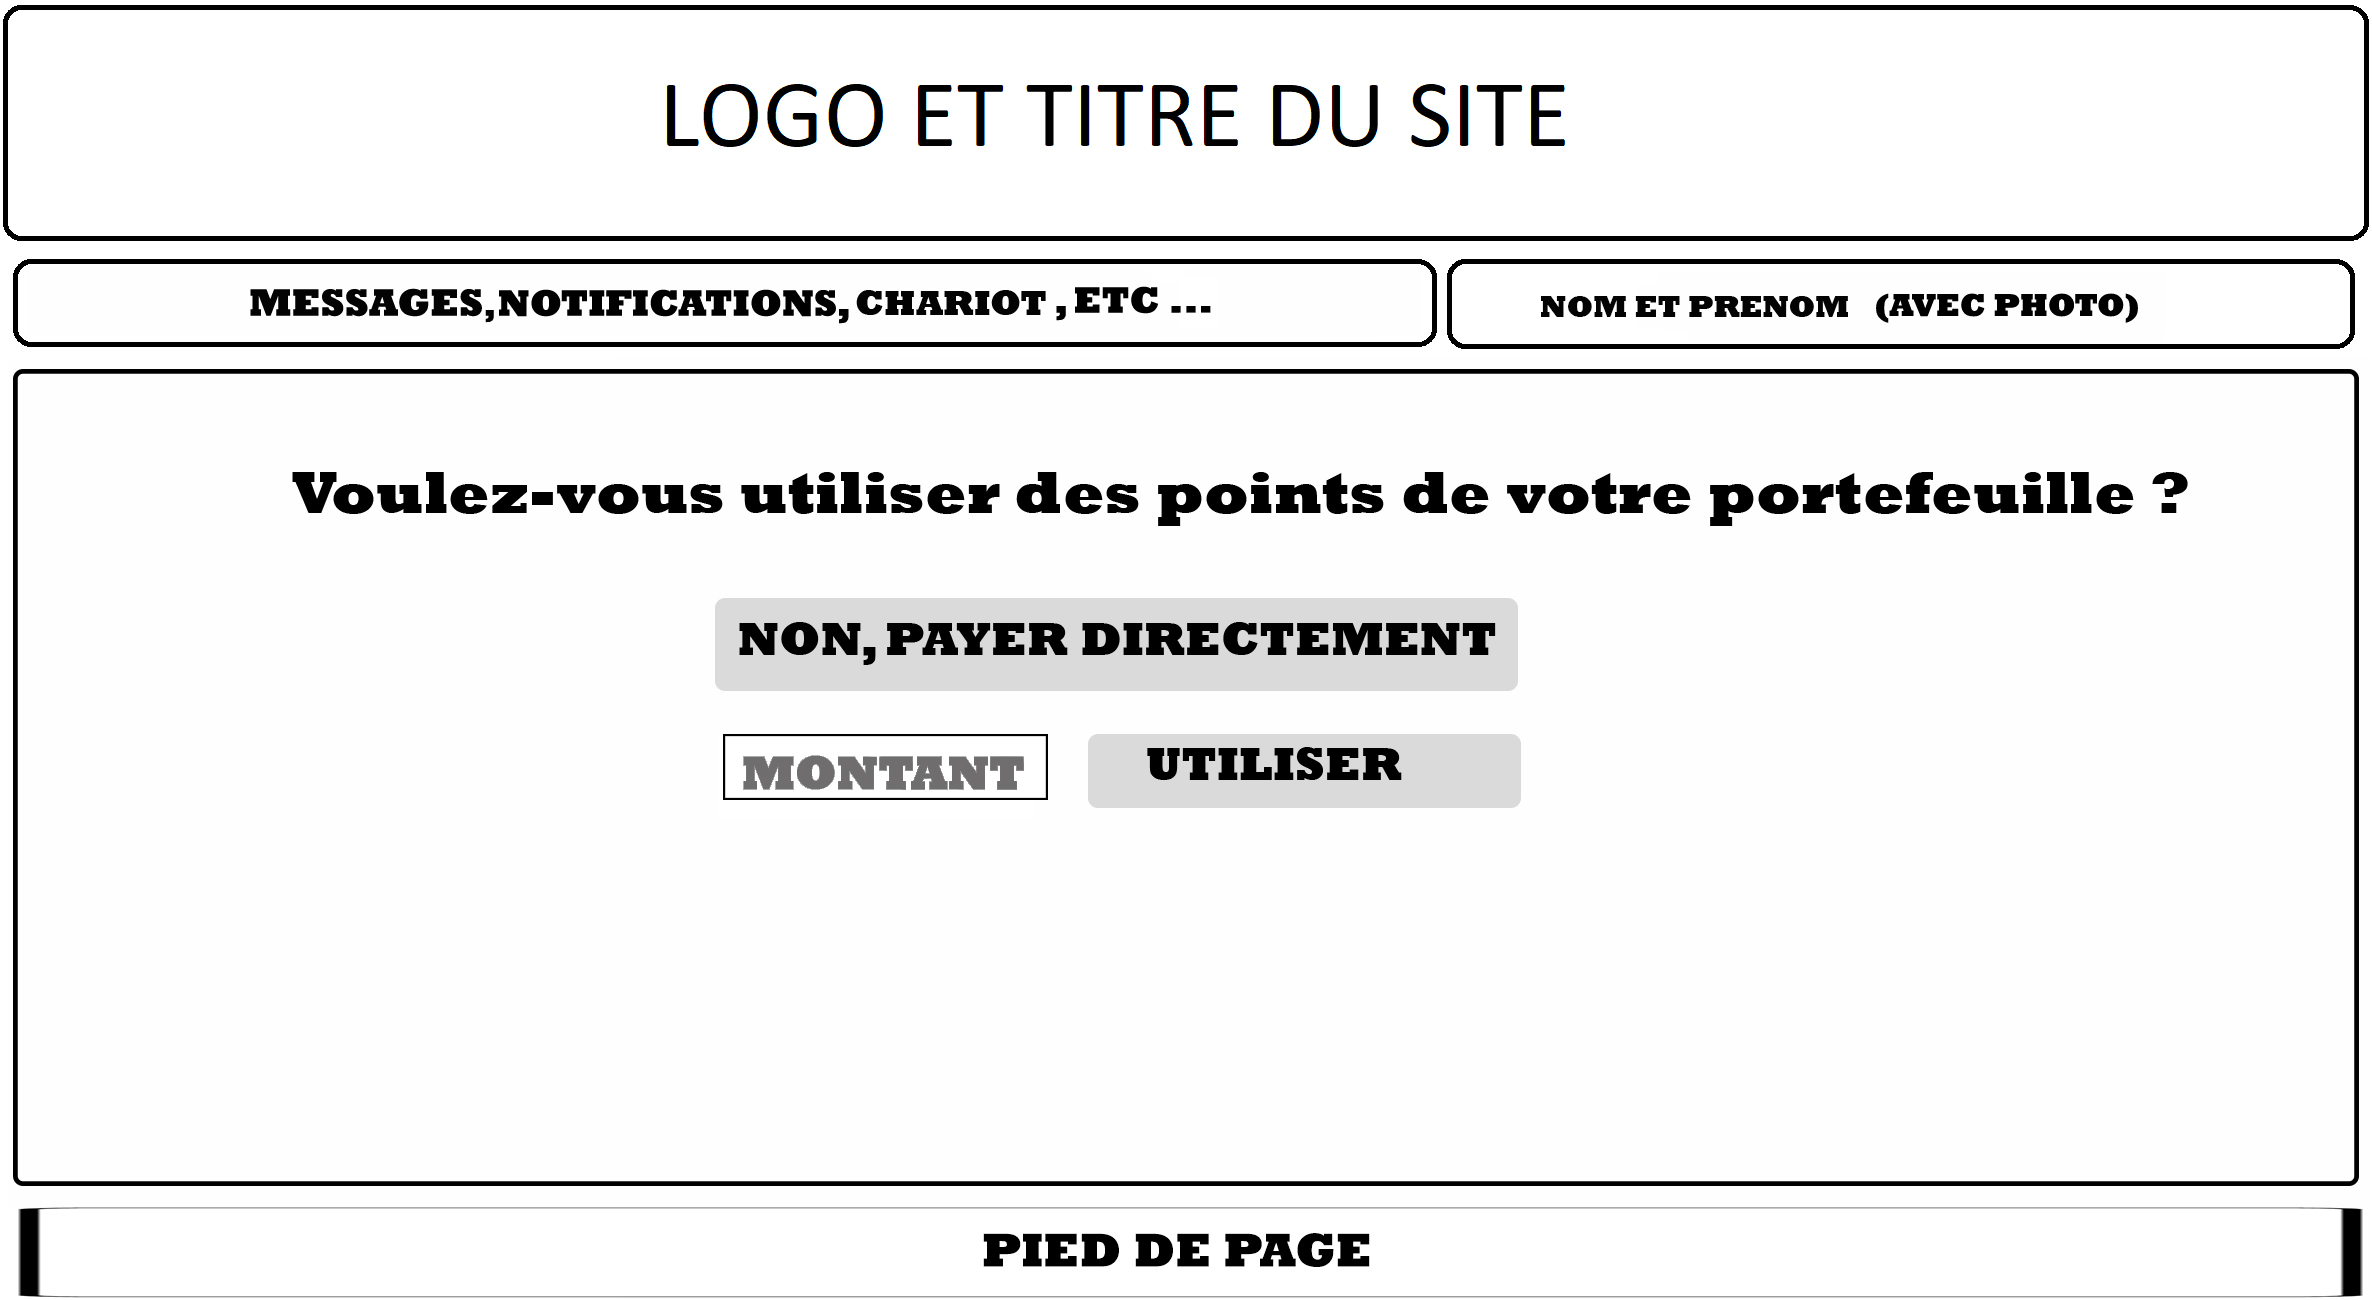
\includegraphics[scale=0.25]{images/storyboard/04_3.jpg}
  \caption{Règlement d'achat}
\end{figure}

\begin{figure}[!ht]
  \centering
  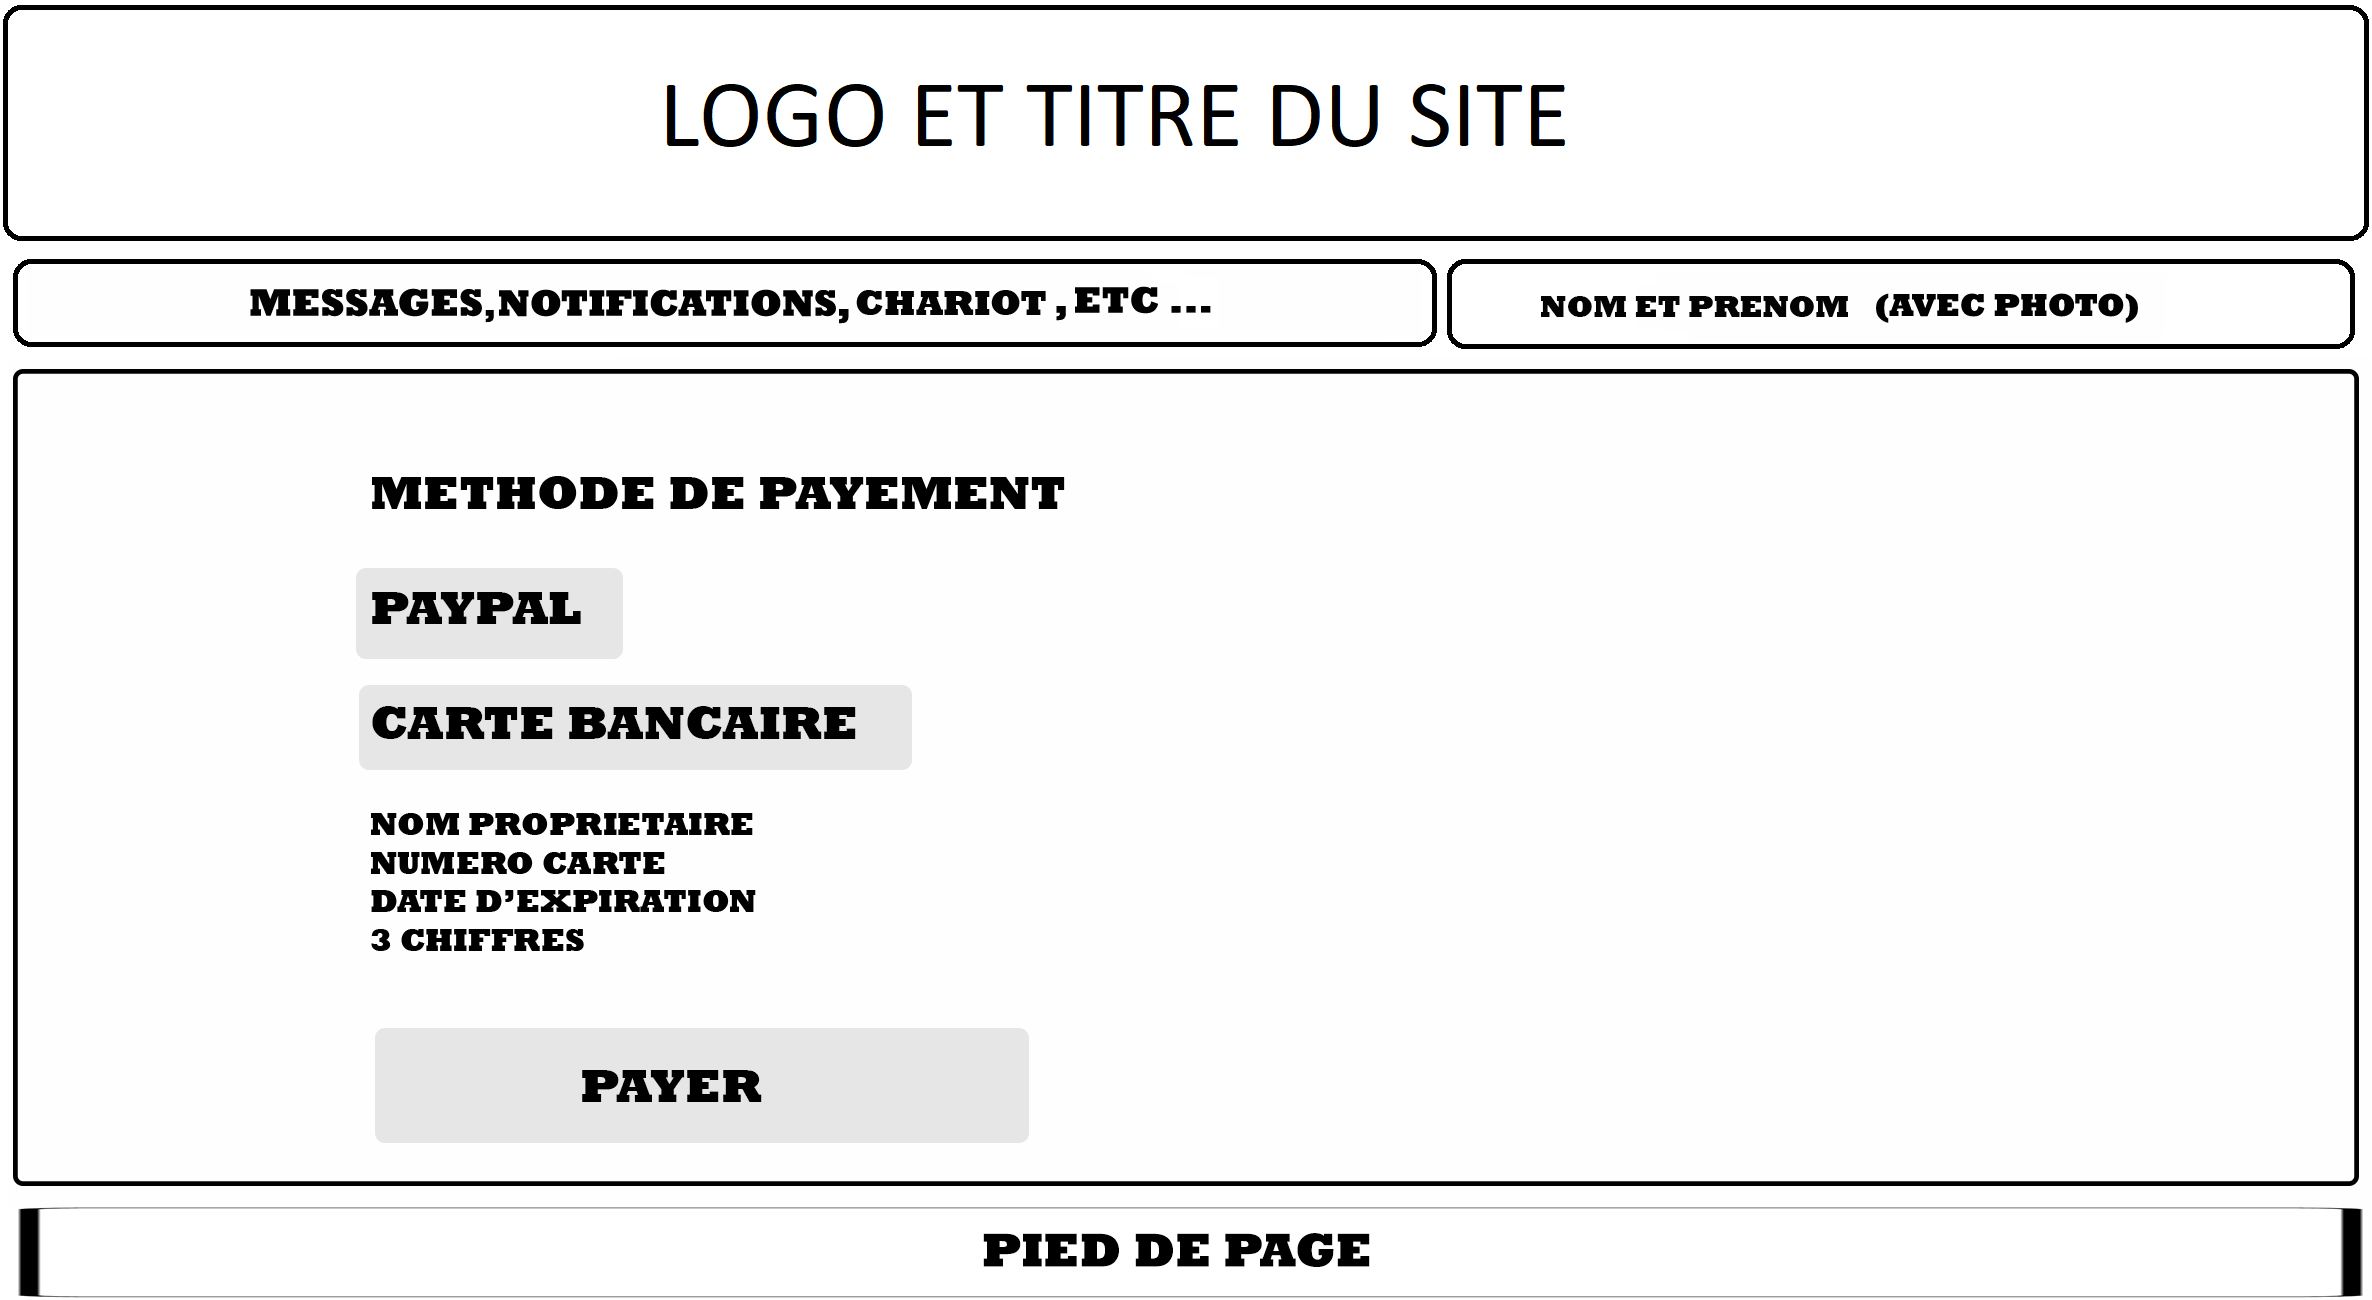
\includegraphics[scale=0.25]{images/storyboard/04_4.jpg}
  \caption{Méthodes de paiement}
\end{figure}

\begin{figure}[!ht]
  \centering
  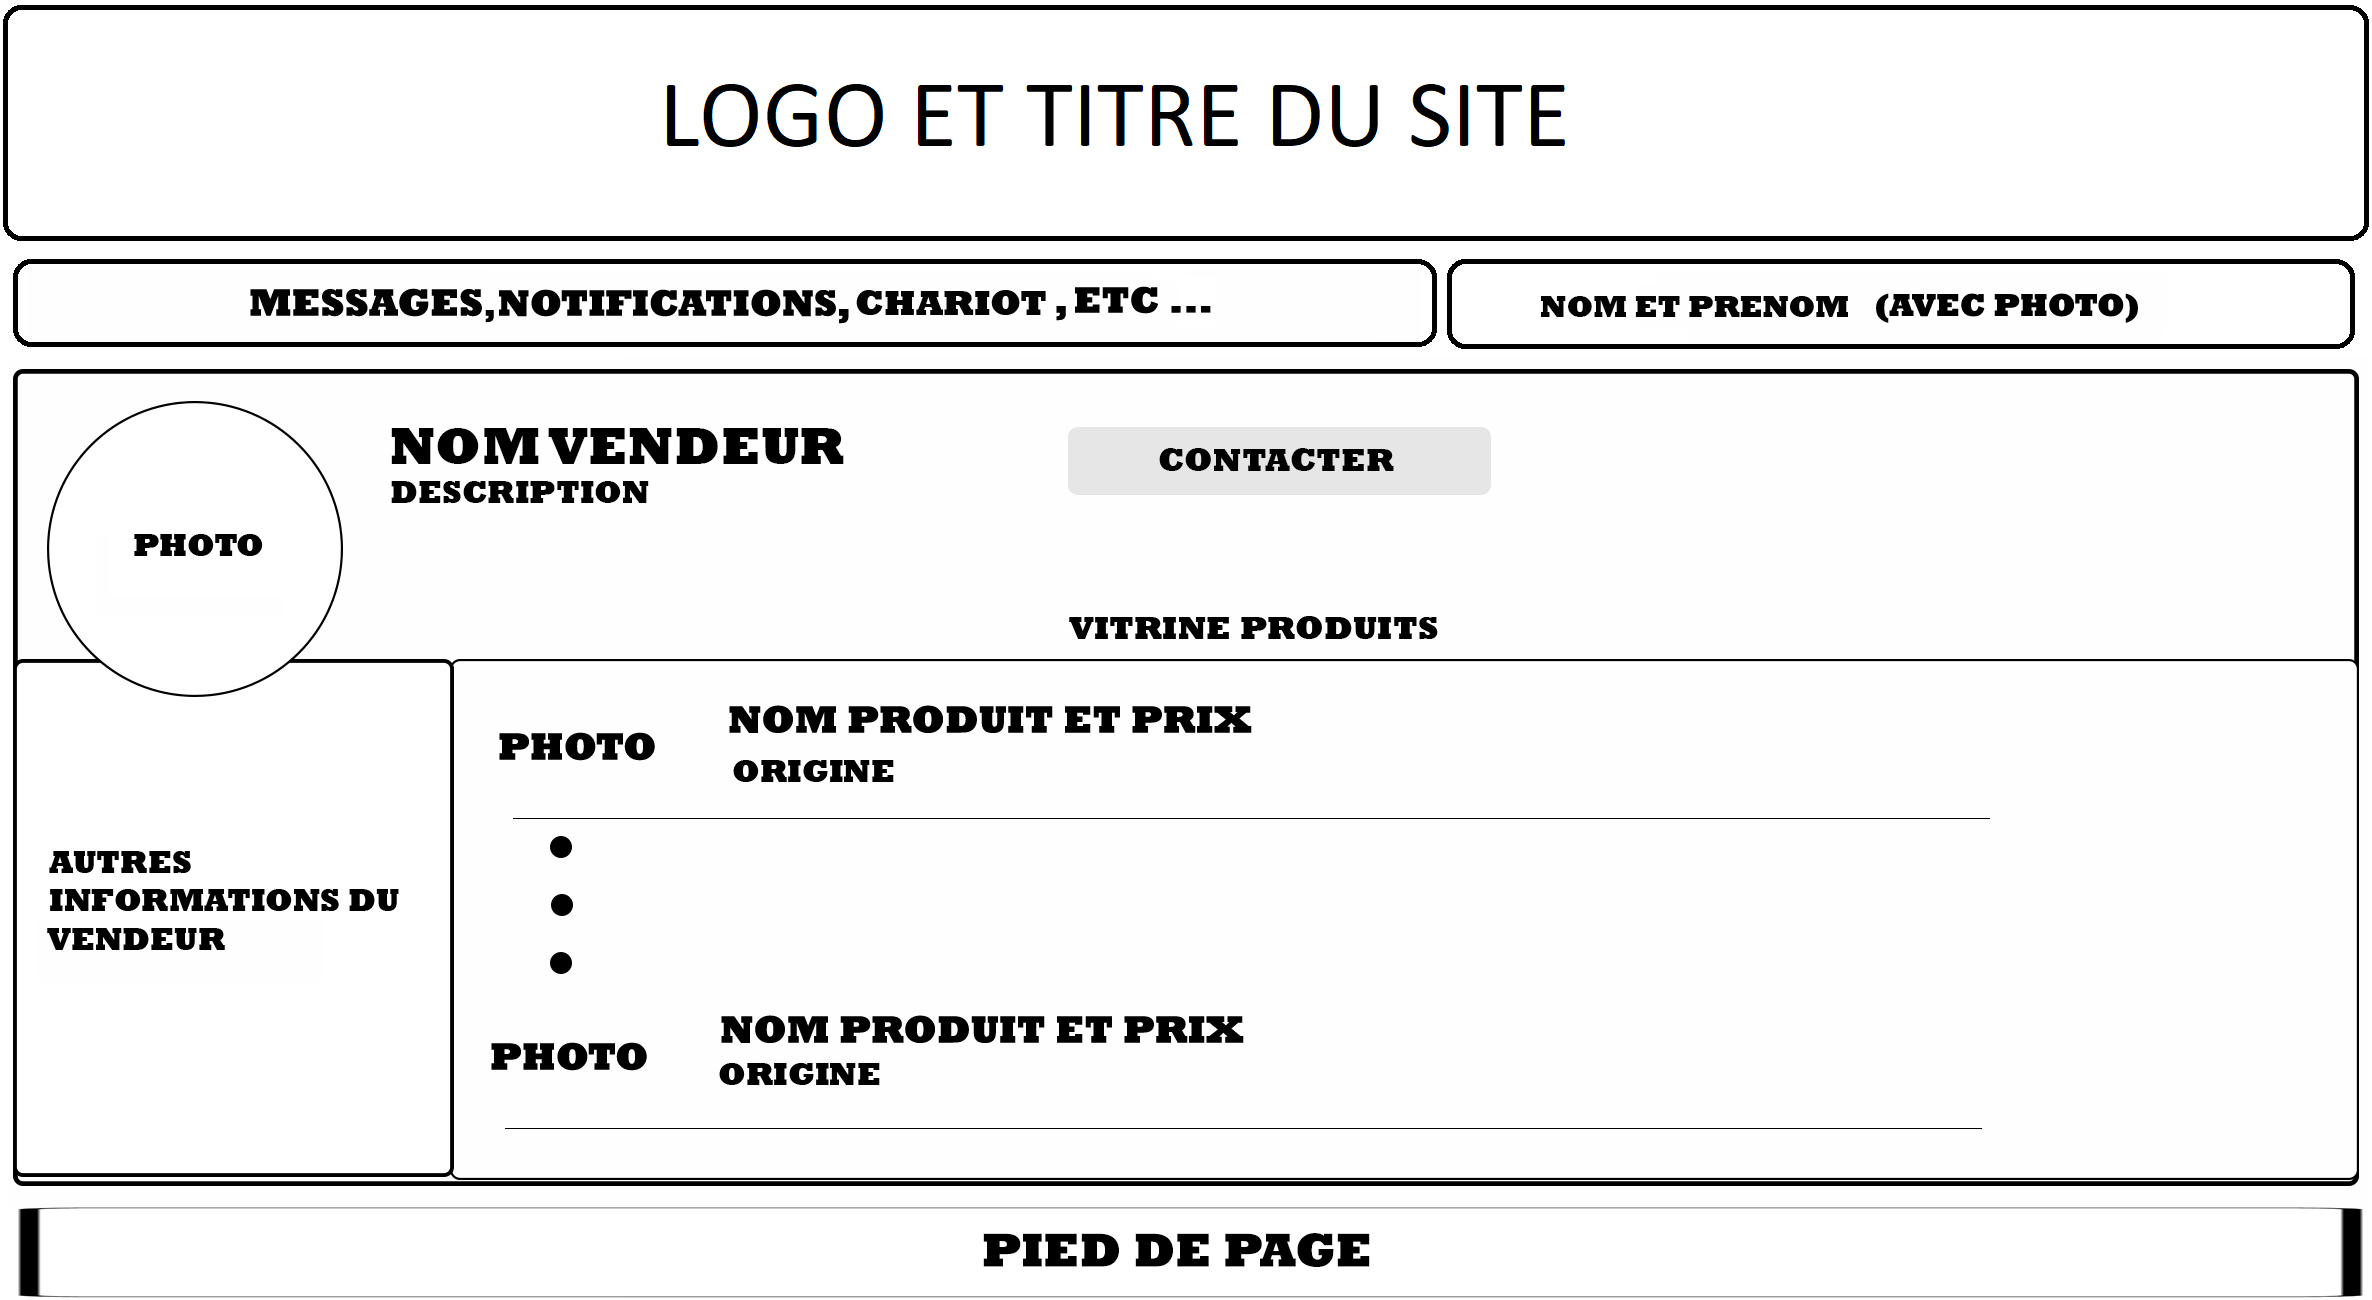
\includegraphics[scale=0.25]{images/storyboard/05.jpg}
  \caption{Informations sur un vendeur}
\end{figure}

\begin{figure}[!ht]
  \centering
  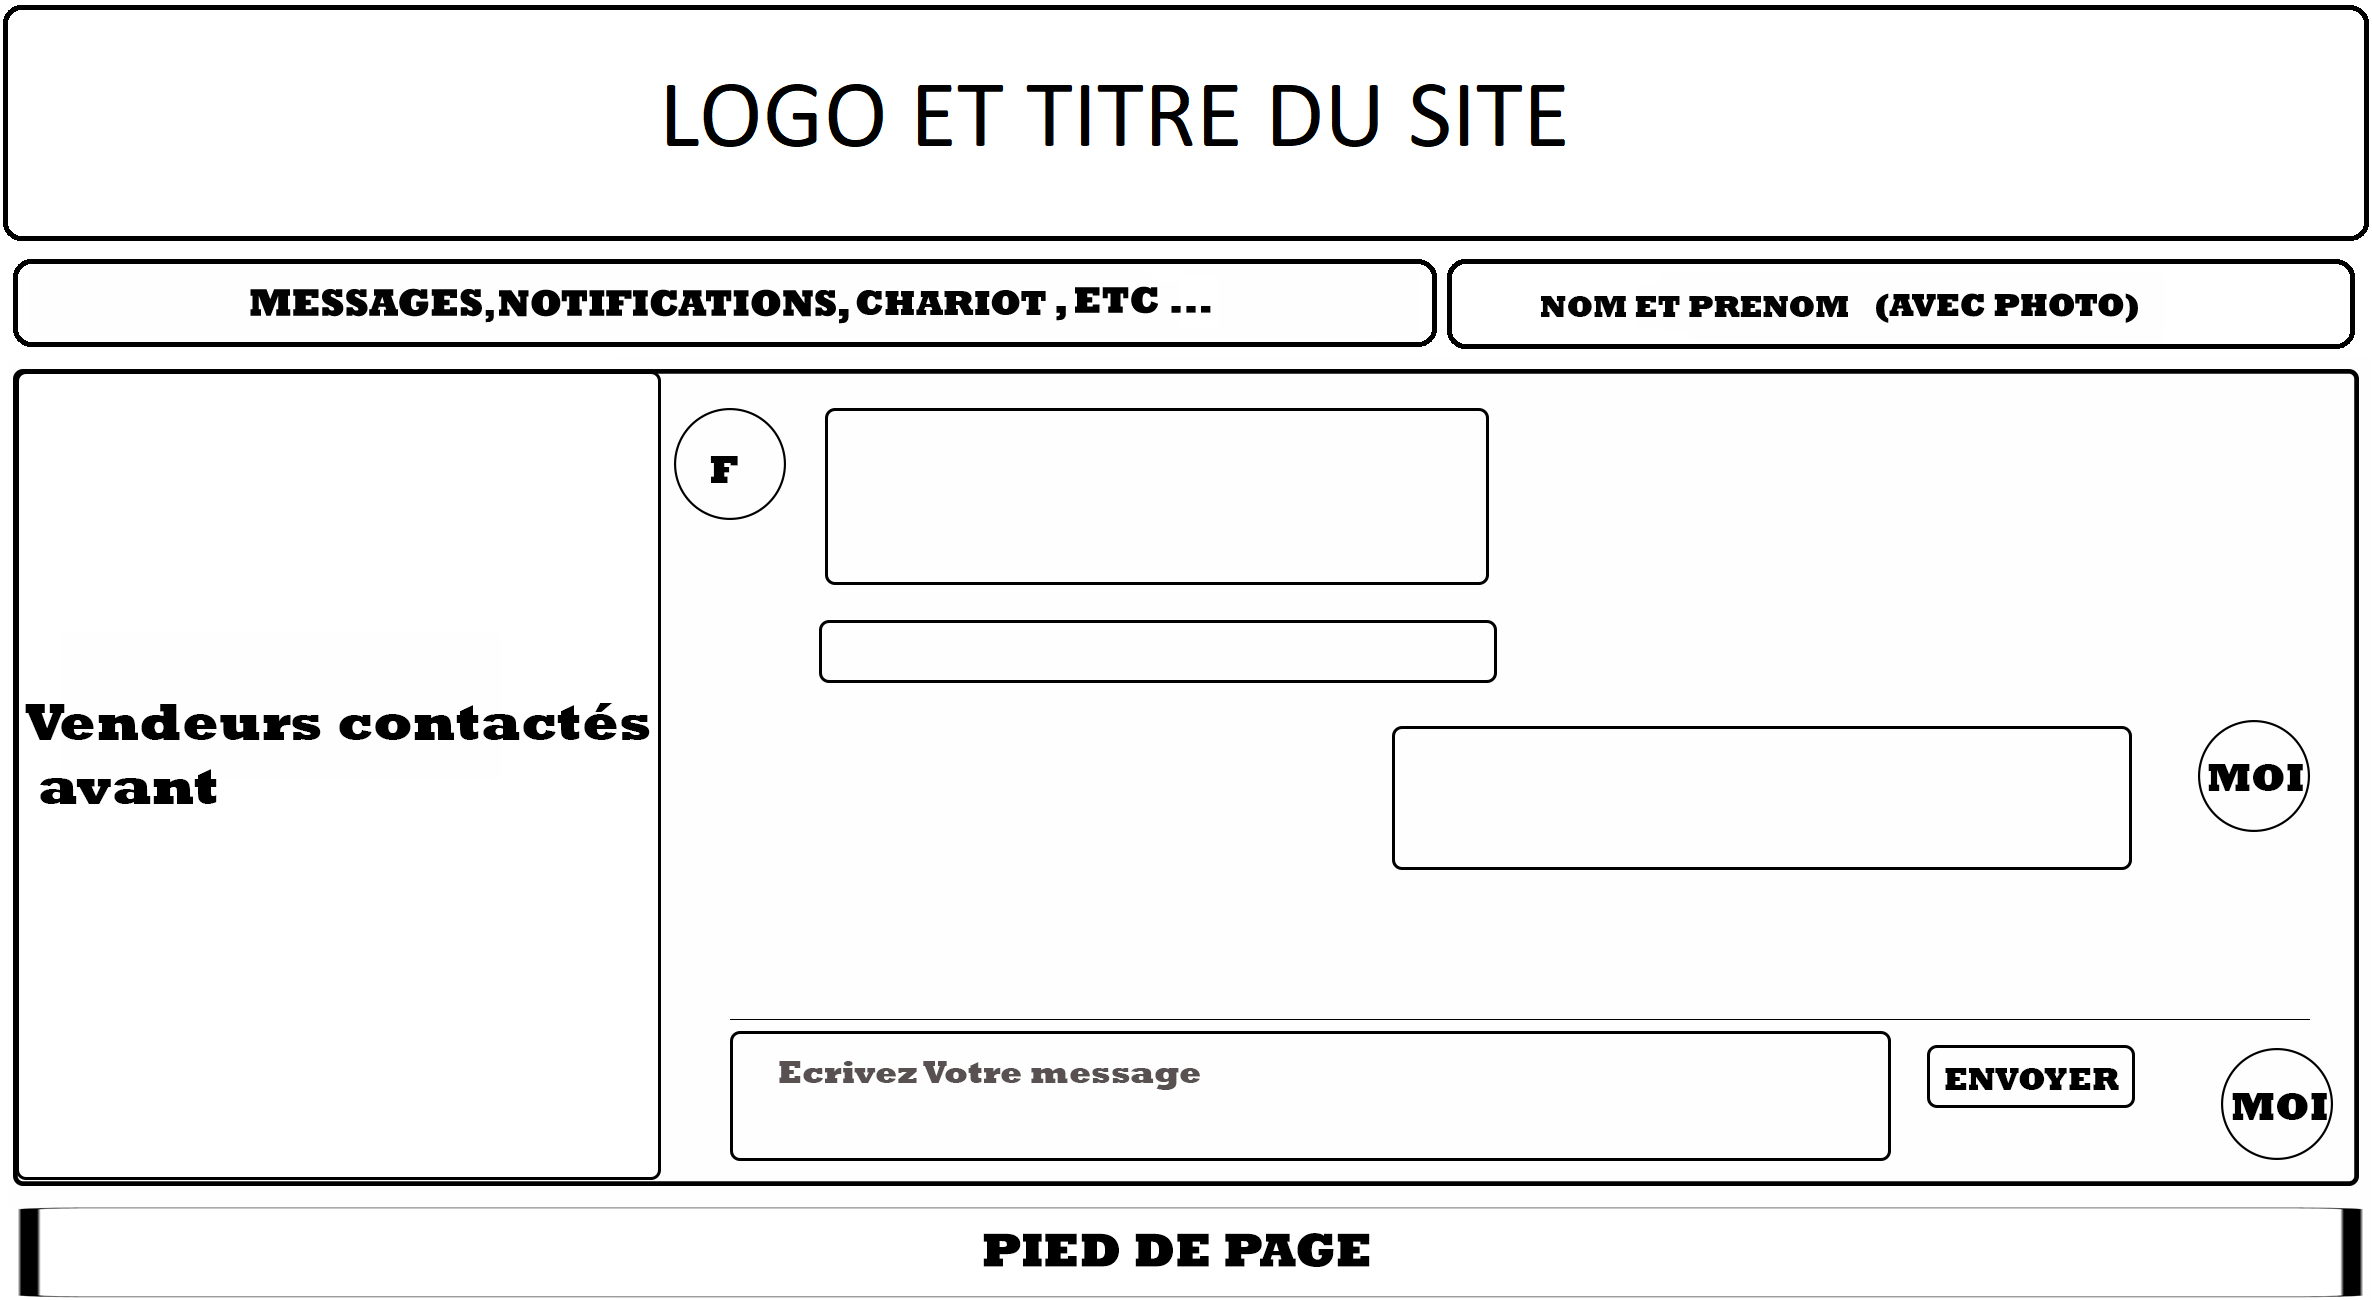
\includegraphics[scale=0.25]{images/storyboard/05_1.jpg}
  \caption{Chat}
\end{figure}

\begin{figure}[!ht]
  \centering
  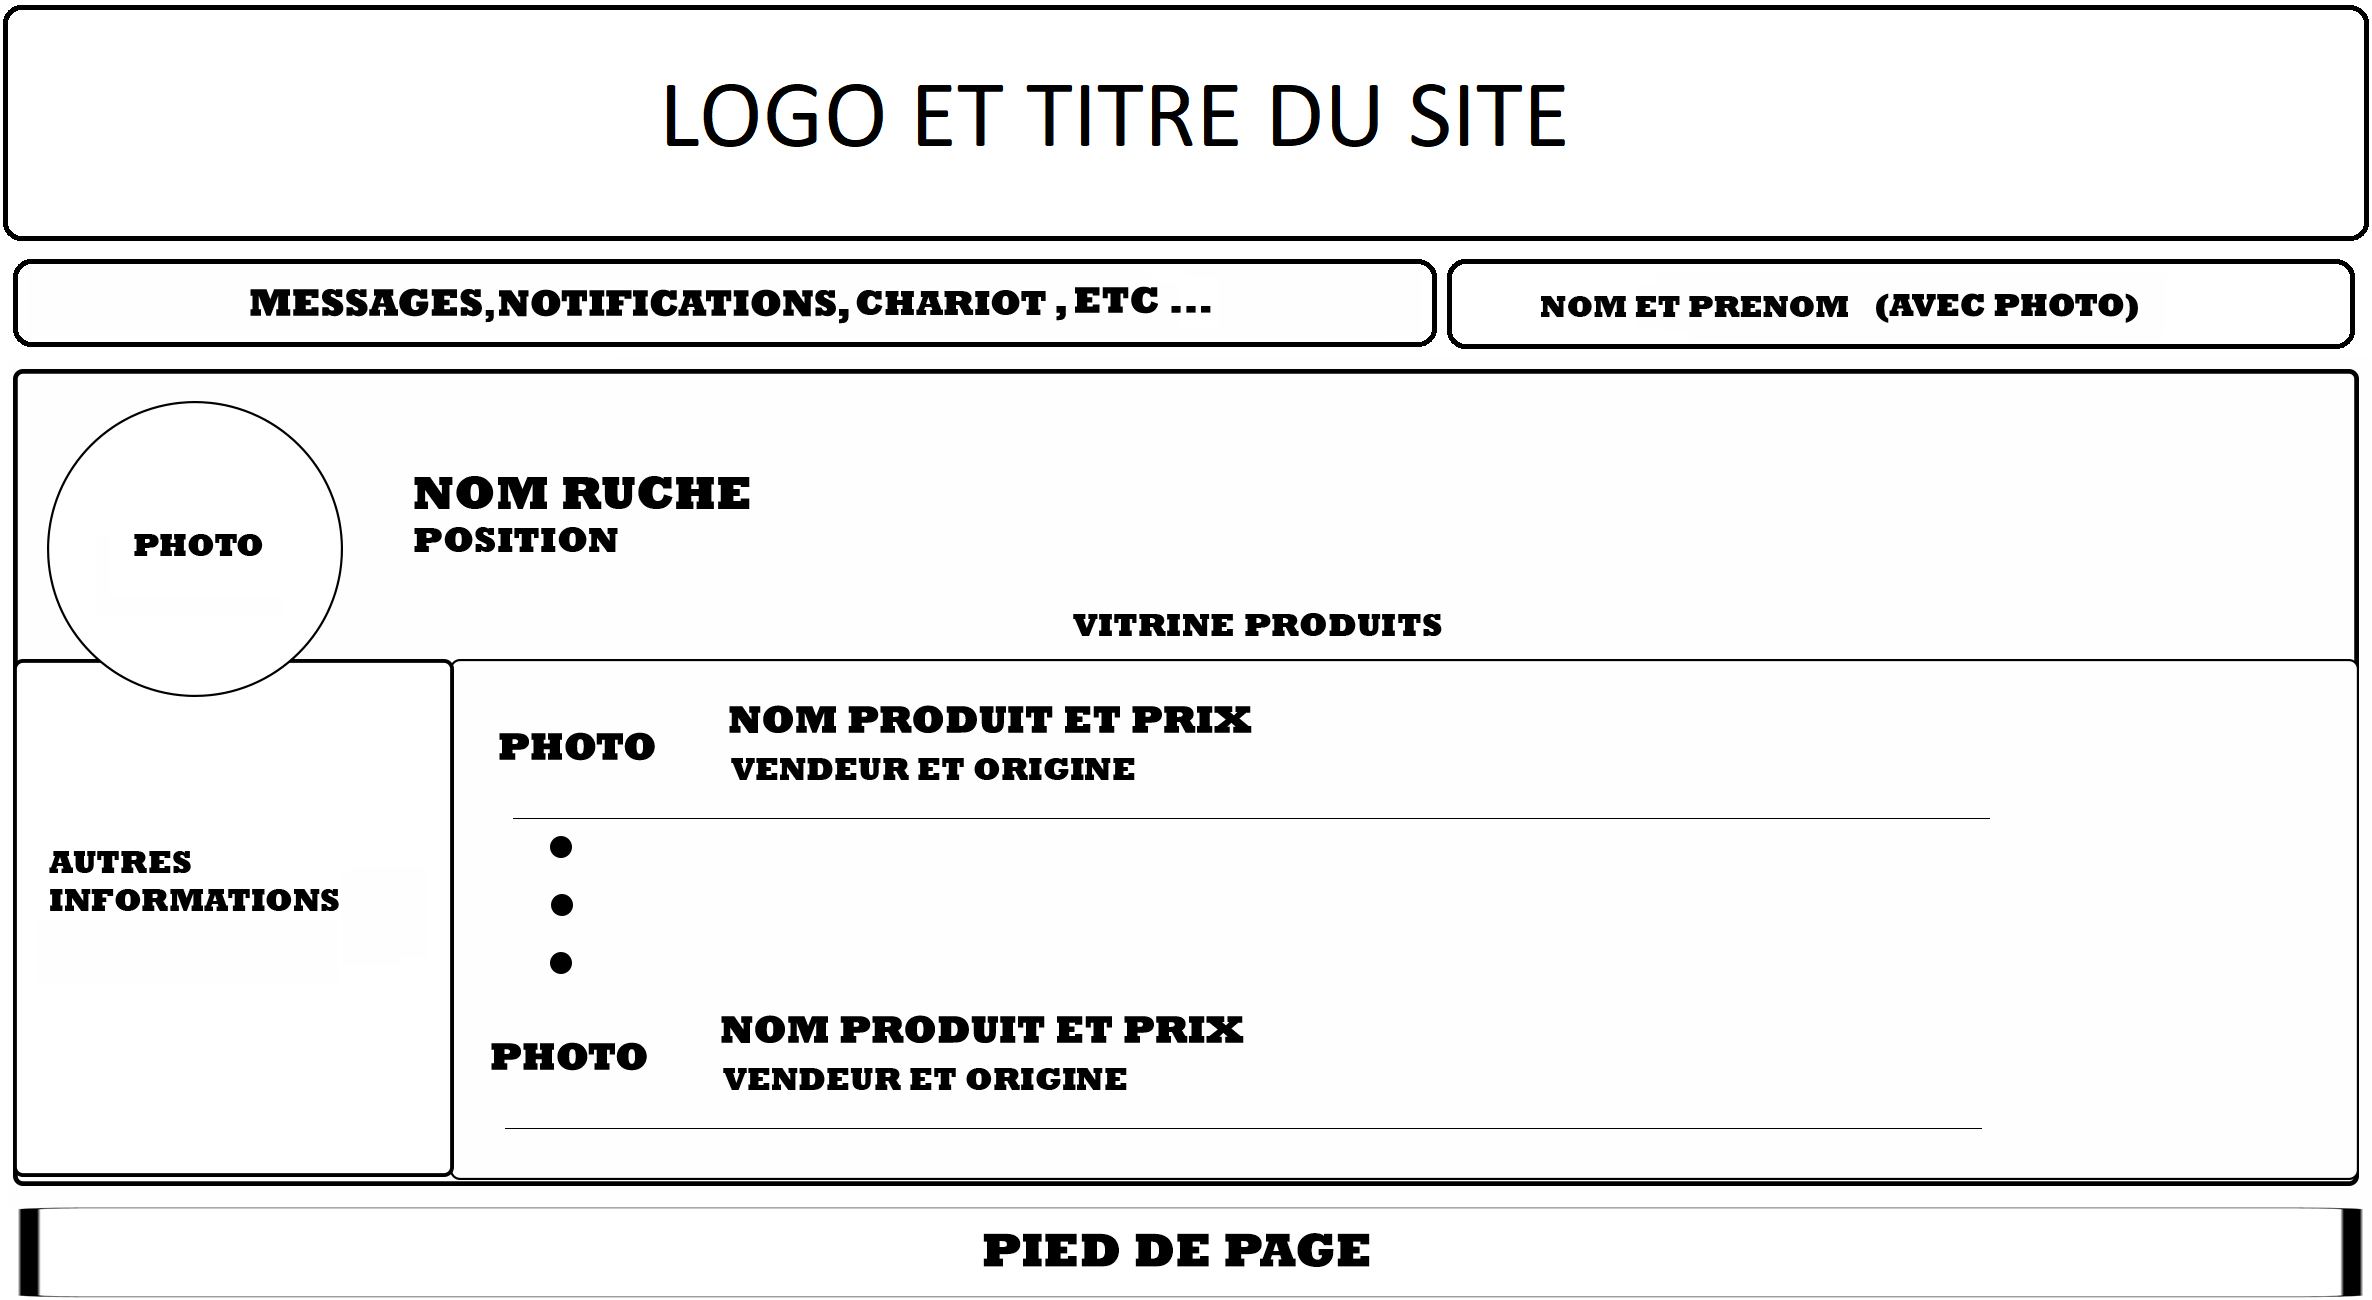
\includegraphics[scale=0.25]{images/storyboard/06.jpg}
  \caption{Informations sur une ruche}
\end{figure}

\begin{figure}[!ht]
  \centering
  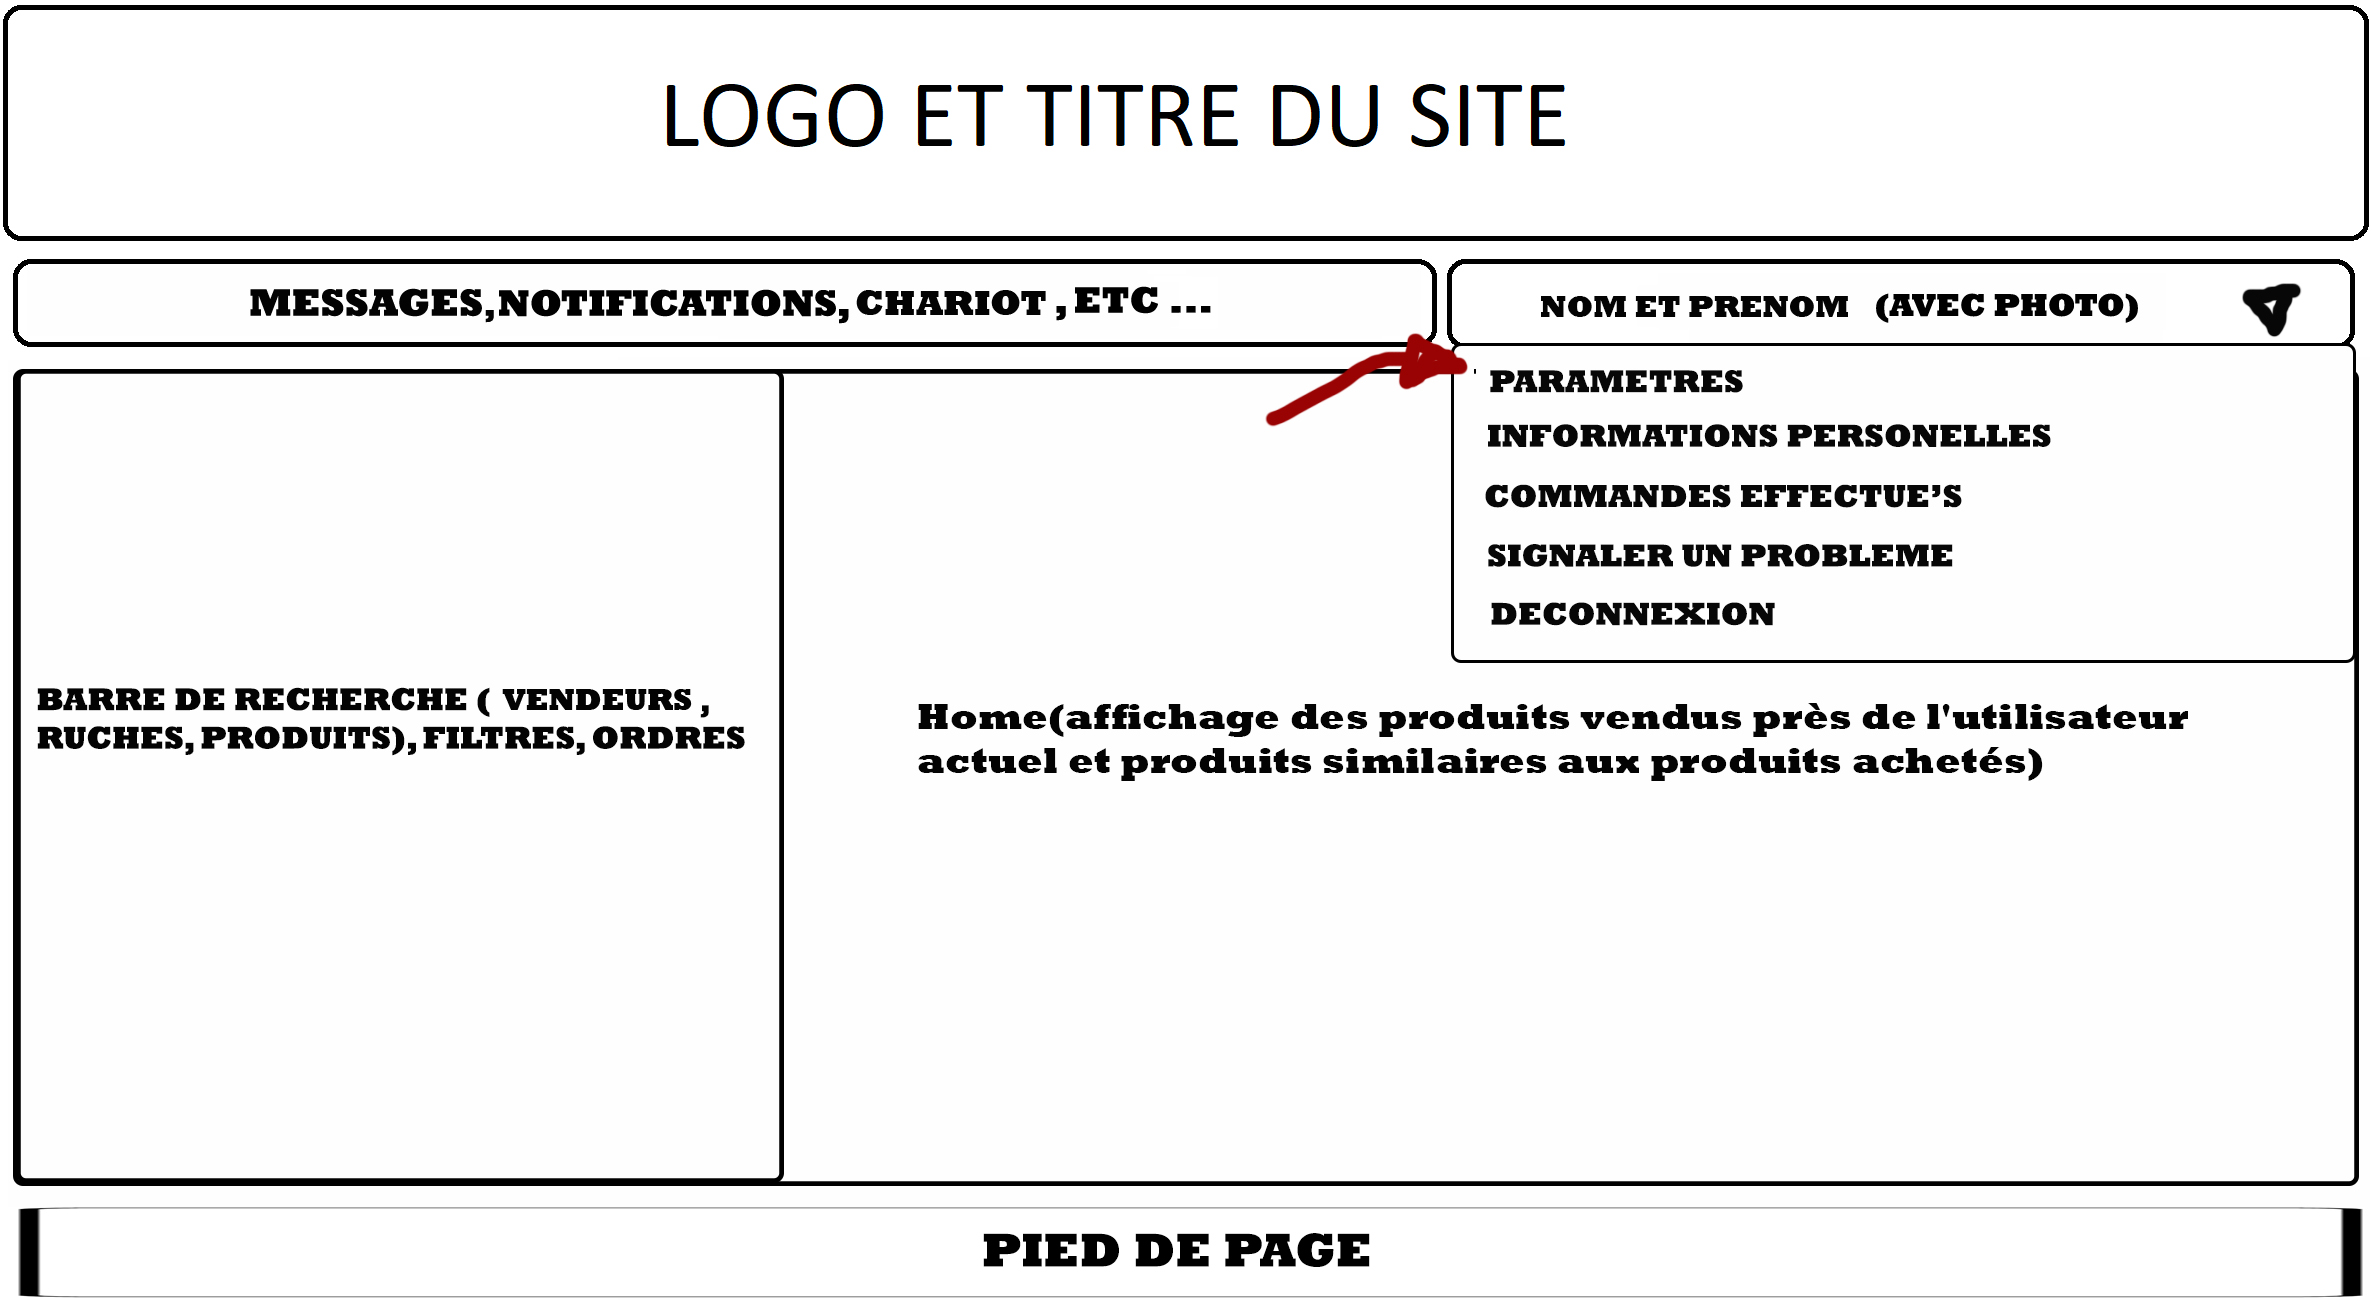
\includegraphics[scale=0.25]{images/storyboard/07.jpg}
  \caption{Barre de paramètres d'un vendeur}
\end{figure}

\begin{figure}[!ht]
  \centering
  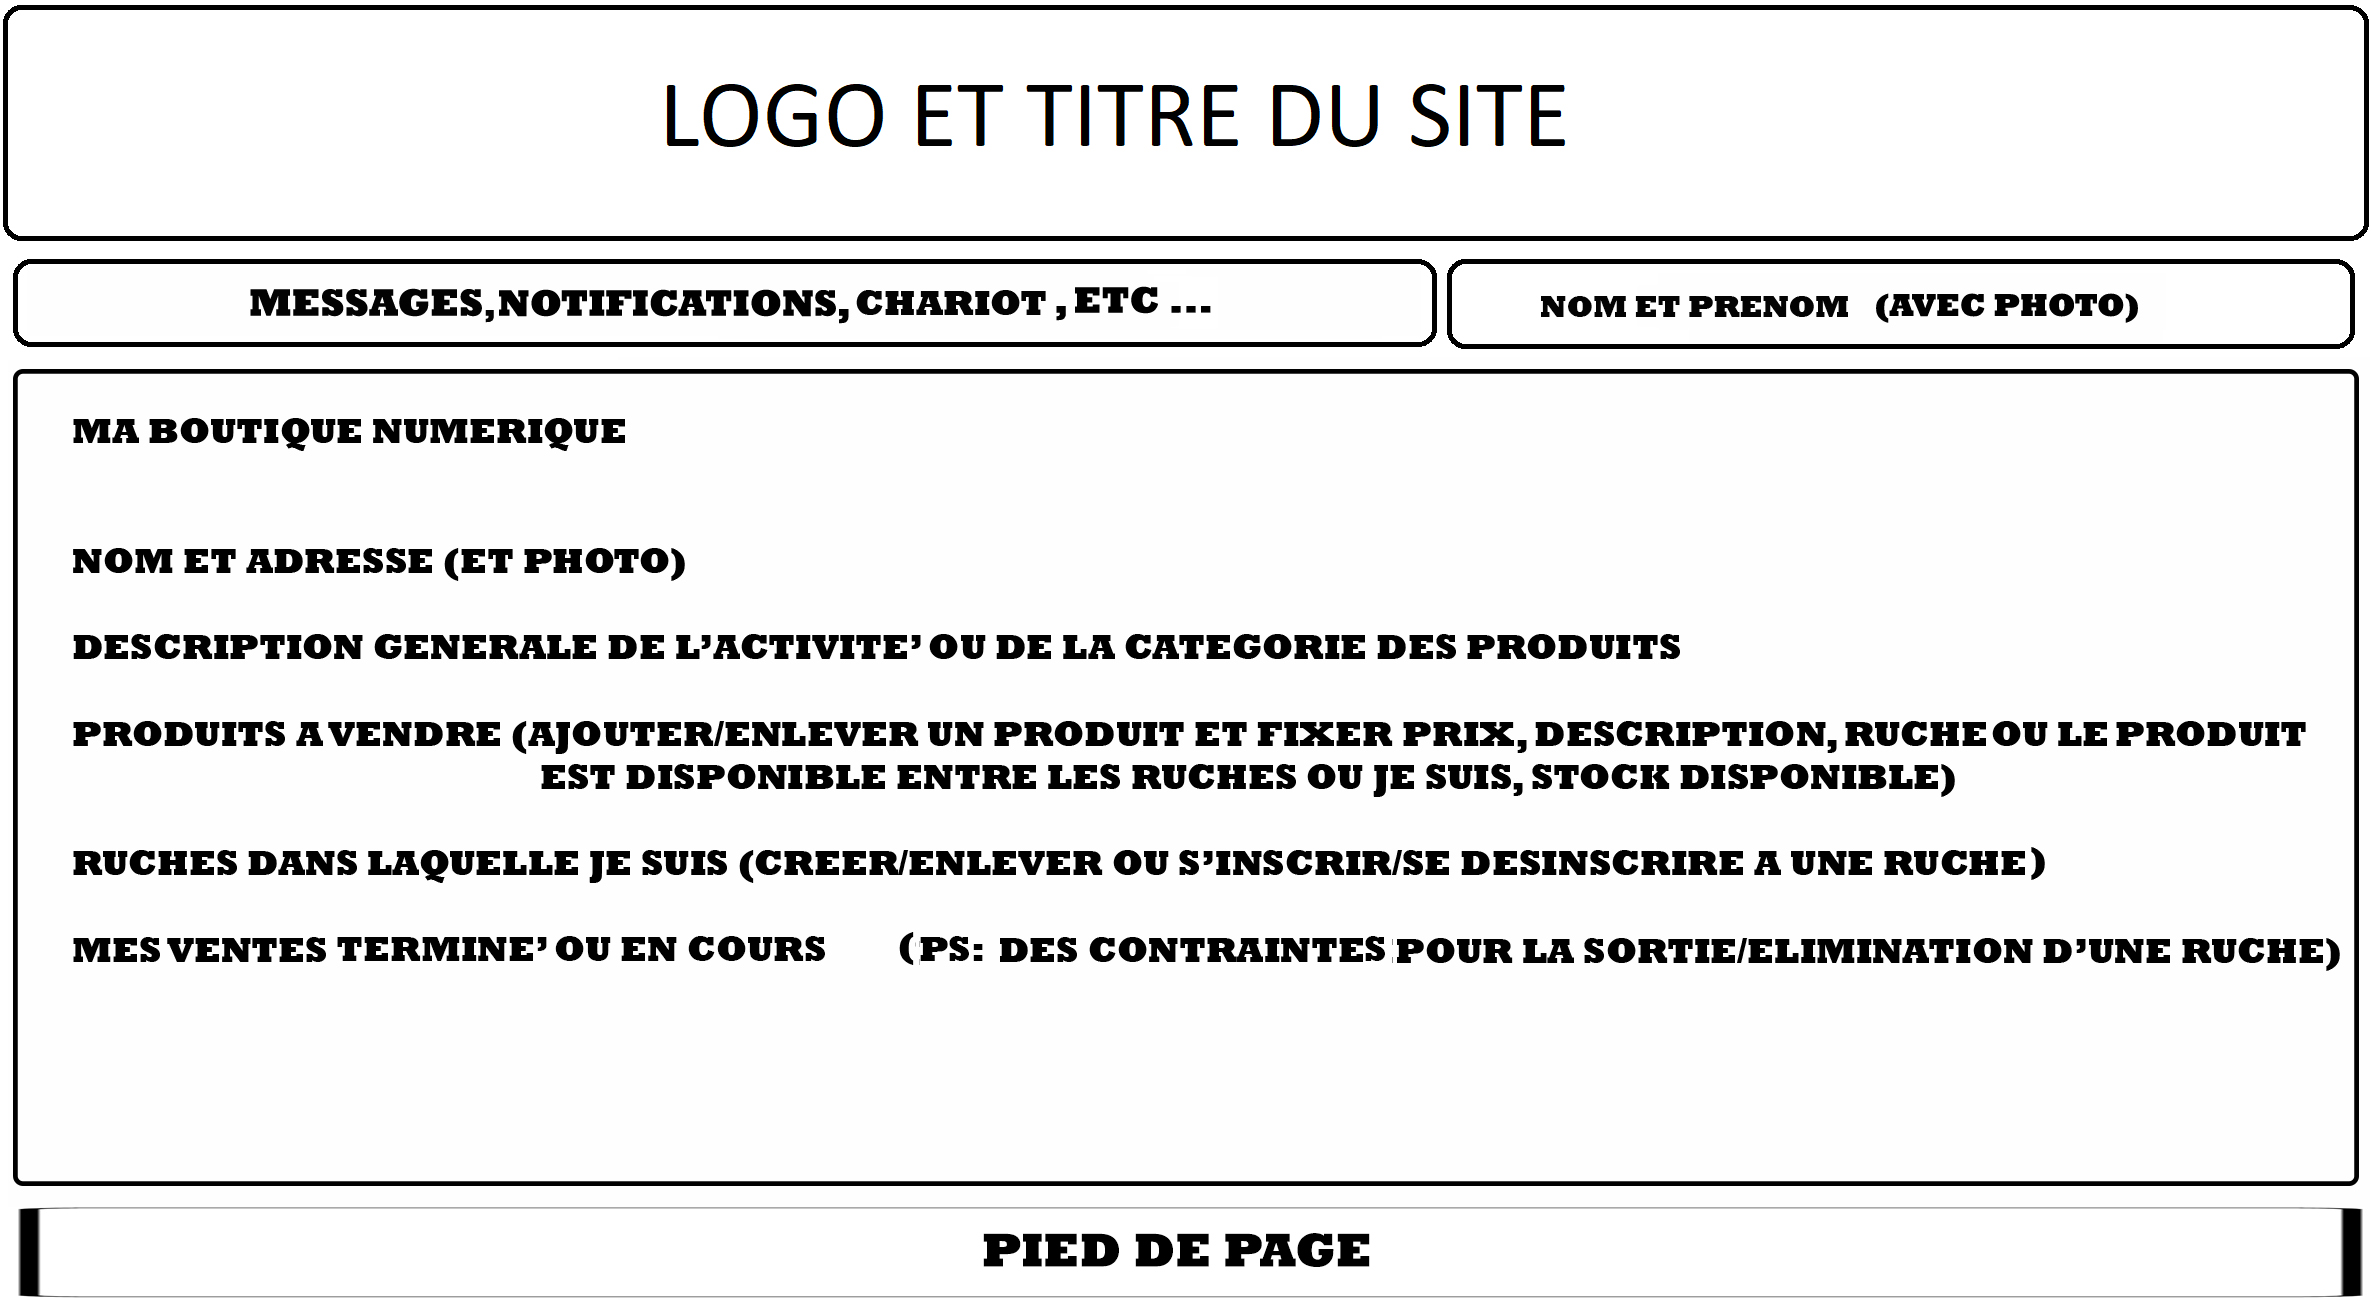
\includegraphics[scale=0.25]{images/storyboard/08.jpg}
  \caption{Barre de paramètres du compte d'un vendeur}
\end{figure}
\end{appendices}
%----------------------------------------------------------------------------------------
%   BIBLIOGRAPHIE
%----------------------------------------------------------------------------------------
\bibliographystyle{agsm}
\bibliography{mybib}
\end{document}
